\documentclass{ctexart}

% if you need to pass options to natbib, use, e.g.:
%     \PassOptionsToPackage{numbers, compress}{natbib}
% before loading neurips\_2019

% ready for submission
%\usepackage{neurips\_2019}

% to compile a preprint version, e.g., for submission to arXiv, add add the
% [preprint] option:
%     \usepackage[preprint]{neurips\_2019}

% to compile a camera-ready version, add the [final] option, e.g.:
\usepackage[final, nonatbib]{neurips\_2020}

\usepackage{pbox}
\usepackage[utf8]{inputenc} % allow utf-8 input
\usepackage{hyperref}       % hyperlinks
\usepackage{url}            % simple URL typesetting
\usepackage{booktabs}       % professional-quality tables
\usepackage{multirow}
\usepackage{amsfonts}       % blackboard math symbols
\usepackage{amsmath}
\usepackage{graphicx,wrapfig,lipsum}
\usepackage{amsfonts}
\usepackage{booktabs}
\usepackage{empheq}
\usepackage{amsthm}
\usepackage{caption}
\usepackage{subcaption}
\usepackage{mathrsfs}  
\usepackage{amssymb}
\usepackage{thmtools}  % restatable
\usepackage{tikz}
\usepackage{nicefrac}
\usepackage{arydshln}
\usetikzlibrary{calc,positioning,matrix, decorations.pathreplacing}

%\usepackage{nicefrac}       % compact symbols for 1/2, etc.
%\usepackage{microtype}      % microtypography
%\usepackage[title]{appendix}

\hyphenpenalty=10000

\theoremstyle{plain}
\newtheorem{thm}{Theorem}[section]
\newtheorem*{thm-informal}{Theorem (Informal)}
\newtheorem{proposition}[thm]{Proposition}
\newtheorem{lemma}[thm]{Lemma}
\newtheorem{corollary}[thm]{Corollary}

\theoremstyle{definition}
\newtheorem{definition}[thm]{Definition}
\newtheorem{remark}[thm]{Remark}
\newtheorem{example}[thm]{Example}


\newcommand{\ts}[2]{\mathcal{T\!S}\_{#1}\left(#2\right)}
\newcommand{\norm}[1]{\left\|#1\right\|}
\newcommand{\abs}[1]{\left|#1\right|}
\newcommand{\reals}{\mathbb{R}}
\newcommand{\naturals}{\mathbb{N}}
\newcommand{\bigO}{\mathcal{O}}
%\newcommand{\ttfrac}[2]{\null^{#1}\!/\_{#2}}
\newcommand{\ttfrac}[2]{\nicefrac{#1}{#2}}
\newcommand{\set}[2]{\left\{{#1}\,\left\vert\,{#2}\vphantom{{#1}}\right\}\right.}
\newcommand{\score}[2]{#1\% $\pm$ #2\%}
\newcommand{\bfscore}[2]{\textbf{#1\%} $\mathbf{\pm}$ \textbf{#2\%}}
\newcommand{\aucscore}[2]{#1 $\pm$ #2}
\newcommand{\bfaucscore}[2]{\textbf{#1} $\mathbf{\pm}$ \textbf{#2}}
\newcommand{\boldheading}[1]{

\textbf{#1}\quad}

\title{用于不规则时间序列的神经控制微分方程}

%\author{
%	Patrick Kidger$^{1, 2}$
%	\And
%	Cristopher Salvi$^{1, 2}$
%	\And
%	James Morrill$^{1, 2}$
%	\And
%	James Foster$^{1}$
%	\And
%	Terry Lyons$^{1, 2}$
%	\AND \\[-12pt]
%	\null$^1$ Mathematical Institute, University of Oxford \\
%	\null$^2$ The Alan Turing Institute, British Library \\
%	\texttt{\{kidger, salvi, morrill, foster, tlyons\}@\hspace{0.8pt}maths.ox.ac.uk}}
	
\author{Patrick Kidger \qquad James Morrill \qquad James Foster \qquad Terry Lyons\\[2pt]
	Mathematical Institute, University of Oxford \\
	The Alan Turing Institute, British Library \\
	\texttt{\{kidger, morrill, foster, tlyons\}@\hspace{0.8pt}maths.ox.ac.uk}}

\usepackage{titlesec}
\titlespacing*{\section}{0pt}{12pt}{8pt}
\titlespacing*{\subsection}{0pt}{10pt}{6pt}
\titlespacing*{\subsubsection}{0pt}{8pt}{4pt}
\setlength{\parskip}{0.5em}
\setlength{\parsep}{0.5em}
\begin{document}
	\maketitle
\begin{abstract}
		神经常微分方程是建模时间动态的一个有吸引力的选择。然而，一个基本的问题是，常微分方程的解由其初始条件决定，并且没有根据后续观察调整轨迹的机制。在这里，我们通过良好理解的\emph{控制微分方程}数学展示了如何解决这个问题。由此产生的\emph{神经控制微分方程}模型可以直接应用于部分观测的不规则采样多变量时间序列的一般设置中，并且（与之前关于此问题的工作不同）即使在跨观测时也可以利用内存高效的伴随反向传播。我们证明了我们的模型在一系列数据集的经验研究中相对于类似（基于ODE或RNN）模型达到了最先进的性能。最后，我们提供了理论结果，证明了通用逼近性，并表明我们的模型包含了替代的ODE模型。
\end{abstract}
	\section{引言}
	递归神经网络（RNN）是处理序列数据（如时间序列）的一种流行模型选择。数据本身通常被认为是从某个基础过程中得到的一系列观测值，而RNN可以被解释为该过程某函数的离散近似。实际上，RNN和动力系统之间的联系是众所周知的 \cite{FUNAHASHI1993801, rnn-dynamical, E2017, nais-net}。
	
	然而，如果数据是不规则采样的或部分观测的，这种离散化通常会失效，而且这个问题经常通过分箱或插补数据来掩盖 \cite{gelman2007dataanalysis}。
	
	一种更为优雅的方法是认识到，由于底层过程是在连续时间内发展的，因此我们的模型也应该是这样。例如，\cite{Che2018, BRITS, NeuralHawkes, discreteevent} 在观测之间加入了指数衰减，\cite{gp-adapter1, gp-adapter2} 将高斯过程与传统的神经网络模型结合，\cite{interpolation-prediction} 近似了底层的连续时间过程，而 \cite{latent-odes, gru-ode-bayes} 通过允许某些隐藏状态作为ODE演化来适应递归神经网络。正是这最后一点最让我们感兴趣。
	
	\subsection{神经常微分方程}
	神经常微分方程（Neural ODEs）\cite{E2017, neural-odes}，试图通过学习一个函数$f_\theta$和线性映射$\ell^1_\theta$、$\ell^2_\theta$来近似映射$x \mapsto y$，使得
\begin{equation}\label{eq:node}
	y \approx \ell^1_\theta(z_T),\quad\text{where}\quad z_t = z_0 + \int_0^t f_\theta(z_s) \mathrm{d} s\quad\text{and}\quad z_0 = \ell^2_\theta(x).
\end{equation}
	请注意，$f_\theta$并不明确依赖于$s$；如果需要的话，可以将其作为$z_s$中的额外维度包含进去 \cite[Appendix B.2]{neural-odes}。
	
	神经常微分方程是一个优雅的概念。它们提供了机器学习与另一个主导建模范式——微分方程之间的接口。这样做允许应用该领域中已知良好的工具。神经常微分方程还与流形假设完美互动，因为它们描述了沿之演化的数据流形的流动。
	
	这一描述尚未涉及诸如时间序列之类的顺序数据。方程\eqref{eq:node}中的$t$维度被引入然后积分，这只是模型的一个内部细节。
	
	然而，这个额外（人为的）维度的存在引发了这样一个问题：该模型是否可以扩展到诸如时间序列这样的顺序数据激发了这样一个问题：这个模型是否可以扩展到诸如时间序列这样的顺序数据。给定一些有序数据 $(x_0, \ldots, x_n)$，目标是将方程 \eqref{eq:node} 中的 $z_0 = \ell^2_\theta(x)$ 条件扩展为类似于“$z_0 = \ell(x_0), \ldots, z_n = \ell(x_n)$”的条件，以使引入的 $t$ 维度与数据的自然顺序对齐。

主要难点在于方程 \eqref{eq:node} 定义了一个常微分方程；一旦学到了 $\theta$，那么方程 \eqref{eq:node} 的解就由 $z_0$ 处的初始条件决定，并且没有直接机制来结合后来到达的数据 \cite{nais-net}。% 克服这个问题一直是至今为止几项工作的重点。

%\cite{latent-odes} 和 \cite{gru-ode-bayes} 都通过交错使用神经 ODE 和循环单元来解决这个问题；ODE 决定了观测之间的演变，而循环单元在每次观测时执行更新。不幸的是，这样做不能完全利用由 \cite{neural-odes} 提倡的伴随反向传播，因为每次观测都会中断 ODE。

然而，事实证明，这个问题的解决方案——如何结合传入的信息——已经在数学领域中的粗糙分析中得到了很好的研究，该领域关注于\emph{受控微分方程}的研究。\footnote{不要与名称相似但独立的控制理论领域混淆。} 例如参见 \cite{lyons1998differential, lyons2014rough, hambly2010uniqueness, chevyrev2018signature}。一个极好的介绍是 \cite{levy-lyons}。一本全面的教科书是 \cite{FritzVictoir10}。

我们不会假设读者熟悉受控微分方程或粗糙分析。唯一可能不熟悉的依赖概念是黎曼-斯蒂尔杰斯积分。

\subsection{贡献}
我们展示了如何通过受控微分方程扩展神经 ODE 模型，我们将此称为\emph{神经受控微分方程}（Neural CDE）模型。正如神经 ODE 是 ResNet 的连续模拟一样，Neural CDE 是 RNN 的连续模拟。

Neural CDE 模型具有三个关键特征。首先，它能够处理传入的数据，这些数据可能是不规则采样和部分观察的。其次（与之前关于这个问题的工作不同），即使跨越观测点，该模型也可以用内存高效的基于伴随的反向传播进行训练。第三，在 CharacterTrajectories、PhysioNet 败血症预测和 Speech Commands 数据集上的实证研究中，它展示了相对于类似（基于 ODE 或 RNN）模型的最先进性能。cal 研究在 CharacterTrajectories、PhysioNet 脓毒症预测和 Speech Commands 数据集上进行。

	我们提供了额外的理论结果，表明我们的模型是一个通用逼近器，并且它包含了表面上类似的 ODE 模型，在这些模型中向量场直接依赖于连续数据。
	
	我们的代码可以在 \url{https://github.com/patrick-kidger/NeuralCDE} 获取。我们也发布了一个库 \texttt{torchcde}，位于 \url{https://github.com/patrick-kidger/torchcde}
	
	\section{背景}
	设 $\tau, T \in \reals$ 且 $\tau < T$，以及 $v, w \in \naturals$。设 $X \colon [\tau, T] \to \reals^v$ 是一个有界变差的连续函数；例如，如果 $X$ 是 Lipschitz 的，则满足此条件。设 $\zeta \in \reals^w$。设 $f \colon \reals^w \to \reals^{w \times v}$ 是连续的。
	
	那么我们可以定义一个连续路径 $z \colon [\tau, T] \to \reals^w$ 通过 $z_\tau = \zeta$ 和
\begin{equation}\label{eq:cde}
	z_t = z_\tau + \int_\tau^t f(z_s) \mathrm{d} X_s\quad\text{for $t \in (\tau, T]$},
\end{equation}
	其中积分是 Riemann--Stieltjes 积分。由于 $f(z_s) \in \reals^{w \times v}$ 和 $X_s \in \reals^v$，记号 ``$f(z_s) \mathrm{d}X_s$'' 指的是矩阵-向量乘法。下标表示函数求值，这在随机微积分中很常见。
	
	方程 \eqref{eq:cde} 在 $f$ 满足全局 Lipschitz 条件时表现出全局存在性和唯一性；参见 \cite[Theorem 1.3]{levy-lyons}。我们称方程 \eqref{eq:cde} 为由 $X$ 控制或驱动的控制微分方程 (CDE)。
	
	% TODO: 删掉这一段？
	%为了提供上下文，考虑随机微分方程 (SDEs) 和 ODEs 之间的区别。SDEs 引入了三个新概念：通过布朗运动控制微分方程、关于无限变差路径的积分（再次是布朗运动）以及随机性。尽管 `SDE' 这个名字只反映了最后一点！相比之下，CDEs 单独实现了第一个概念，而粗糙微分方程 (RDEs) 引入了第二个概念 \cite{levy-lyons}。\footnote{注意许多文献将 `CDE' 和 `RDE' 互换使用。}
	
	\section{方法}	
	假设我们有一个完全观测但可能是不规则采样的时间序列 $\mathbf{x} = ((t_0, x_0), (t_1, x_1), \ldots, (t_n, x_n))$，每个 $t_i \in \reals$ 是观测 $x_i \in \reals^v$ 的时间戳，并且 $t_0 < \cdots < t_n$。（稍后我们将考虑部分观测的数据。）
	
	设 $X \colon [t_0, t_n] \to \reals^{v + 1}$ 是在结点 $t_0, \ldots, t_n$ 处的自然三次样条，使得 $X_{t_i} = (x_i, t_i)$。由于 $\mathbf{x}$ 通常被认为是某个潜在过程的离散化，仅通过 $\mathbf{x}$ 观测到，因此 $X$ 是对该潜在过程的一种近似。自然三次样条具有处理某些边缘情况所需的最小正则性；详见附录 \ref{appendix:other-schemes-for-x} 中的技术细节。
		
	设 $f_\theta \colon \reals^w \to \reals^{w \times (v + 1)}$ 是任何依赖参数 $\theta$ 的神经网络模型。值 $w$ 是描述隐藏状态大小的超参数。设 $\zeta_\theta \colon \reals^{v + 1} \to \reals^w$ 是任何依赖参数 $\theta$ 的神经网络模型。
	
	然后我们定义 \emph{神经控制微分方程} 模型为 CDE
\begin{equation}\label{eq:ncde}
	z_t = z_{t_0} + \int_{t_0}^t f_\theta(z_s) \mathrm{d} X_s\quad\text{for $t \in (t_0, t_n]$},
\end{equation}
	其中 $z_{t_0} = \zeta_\theta(x_0, t_0)$。这个初始条件用于避免平移不变性。类似于 RNNs，模型的输出可以是演化过程 $z$ 或终端值 $z_{t_n}$，并且最终预测通常应通过对此输出应用线性映射来给出。
	
	方程 \eqref{eq:node} 和 \eqref{eq:ncde} 之间的相似性是显而易见的。被引导至这个输出。

公式\eqref{eq:node}和\eqref{eq:ncde}之间的相似性是显而易见的。关键的区别在于，公式\eqref{eq:ncde}是由数据过程$X$驱动的，而公式\eqref{eq:node}仅由恒等函数$\iota \colon \reals \to \reals$驱动。这样，神经CDE自然地适应了传入的数据，因为$X$的变化改变了系统的局部动态。参见图\ref{figure:picture}。

\newcommand{\mainpicturedata}{
	% 时间轴
	\draw[thick,->] (-1, 0)--(5, 0);
	\node at (0, 0)[circle,fill, inner sep=1.5pt]  {};
	\node at (0.6, 0)[circle,fill, inner sep=1.5pt]  {};
	\node at (2, 0)[circle,fill, inner sep=1.5pt]  {};
	\node at (4, 0)[circle,fill, inner sep=1.5pt]  {};
	\node at (0,-0.3) {$t_1$};
	\node at (0.6,-0.3) {$t_2$};
	\node at (2,-0.3) {$t_3$};
	\node at (3,-0.3) {$\cdots$};
	\node at (4,-0.3) {$t_n$};
	\node at (5.6, 0) {时间};
	
	% 数据
	\draw[blue!80!white, thick, cap=round] (-1, 0.3) .. controls ++(45:0.5) and ++(185:0.2) .. (0, 1);
	\draw[blue!80!white, thick, cap=round] (0, 1) .. controls ++(185+180:0.2) and ++(135:0.4) .. (0.6, 0.7);
	\draw[blue!80!white, thick, cap=round] (0.6, 0.7) .. controls ++(135+180:0.4) and ++ (190:0.3) .. (2, 0.6);
	\draw[blue!80!white, thick, cap=round] (2, 0.6) .. controls ++(190+180:0.3) and ++ (135:0.7) .. (4, 0.8);
	\draw[blue!80!white, thick, cap=round] (4, 0.8) .. controls ++(135+180:0.7) and ++(200:0.2) .. (5, 0.6);
	\node at (0, 1)[circle,draw=black, fill=cyan, inner sep=1.5pt] ;
	\node at (0.6, 0.7)[circle,draw=black, fill=cyan, inner sep=1.5pt] ;
	\node at (2, 0.6)[circle,draw=black, fill=cyan, inner sep=1.5pt] ;
	\node at (4, 0.8)[circle,draw=black, fill=cyan, inner sep=1.5pt] ;
	\node at (0, 0.7) {$x_1$};
	\node at (0.6, 0.4) {$x_2$};
	\node at (2, 0.3) {$x_3$};
	\node at (4, 0.5) {$x_n$};
	\node at (5.6, 0.6) {数据$\mathbf{x}$};
	}
\begin{figure}[t]
\begin{subfigure}[b]{0.49\textwidth}\centering
\begin{tikzpicture}[scale=0.9]
	\mainpicturedata
	
	% 隐藏状态
	\draw[olive, thick, cap=round,->] (0, 2)--(0, 1.8);
	\draw[green!80!black, thick, cap=round] (0, 1.8) .. controls (0.3, 1.4) and (0.7, 2.4) .. (0.6,2.2);
	\draw[olive, thick, cap=round,->] (0.6,2.2)--(0.6,1.7);
	\draw[green!80!black, thick, cap=round] (0.6,1.7) .. controls ++(10:0.7) and ++(160:0.6) .. (2,1.9);
	\draw[olive, thick, cap=round,->] (2,1.9)--(2,2.5);
	\draw[green!80!black, thick, cap=round] (2,2.5) .. controls ++(0:0.6) and ++(210:0.9) .. (4,2);
	\draw[olive, thick, cap=round,->] (4,2)--(4, 2.2);
	
	% 更新
	\draw[dashed,->] (0, 1.1)--(0, 1.7);
	\draw[dashed,->] (0.6, 0.8)--(0.6, 1.65);
	\draw[dashed,->] (2, 0.7)--(2, 1.85);
	\draw[dashed,->] (4, 0.9)--(4, 1.95);
	
	\node at (5.6, 2.2) {隐藏状态$z$} {};
\end{tikzpicture}
	%\caption{先前的工作：观察修改隐藏状态。\\}
\end{subfigure}
	\hspace{-0.2em}
\begin{subfigure}[b]{0.49\textwidth}\centering
\begin{tikzpicture}[scale=0.9]
	\mainpicturedata
	
	% 插值数据
	\draw[orange!95!black, thick, cap=round] (0, 2) .. controls ++(0:0.2) and ++(150:0.4) .. (1, 1.7);
	\draw[orange!95!black, thick, cap=round] (1, 1.7) .. controls ++(150+180:0.4) and ++ (185:0.3) .. (2, 1.6);
	\draw[orange!95!black, thick, cap=round] (2, 1.6) .. controls ++(185+180:0.3) and ++ (165:0.7) ..;
	\draw[orange!95!black, thick, cap=round] (2, 1.6) .. controls ++(185+180:0.3) and ++ (165:0.7) .. (4, 1.8);
	\node at (5.6, 1.8) {路径 $X$} {};
	
	% 插值虚线
	\draw[dashed,->] (0, 1.1)--(0, 1.95);
	\draw[dashed,->] (0.6, 0.8)--(0.6, 1.8);
	\draw[dashed,->] (2, 0.7)--(2, 1.55);
	\draw[dashed,->] (4, 0.9)--(4, 1.75);
	
	\draw[dashed,->] (0, 1.1)--(0.4, 1.85);
	\draw[dashed,->] (0.6, 0.8)--(0.2, 1.9);
	\draw[dashed,->] (0.6, 0.8)--(1, 1.65);
	\draw[dashed,->] (0.6, 0.8)--(1.4, 1.5);
	\draw[dashed,->] (0.6, 0.8)--(1.8, 1.5);
	\draw[dashed,->] (2, 0.7)--(1.2, 1.55);
	\draw[dashed,->] (2, 0.7)--(1.6, 1.5);
	\draw[dashed,->] (2, 0.7)--(2.4, 1.6);
	\draw[dashed,->] (4, 0.9)--(3.6, 1.8);
	
	% 隐藏状态
	\draw[green!80!black, thick, cap=round] (0, 3) .. controls ++(-30:0.4) and ++(210:0.5) .. (1, 3);
	\draw[green!80!black, thick, cap=round] (1, 3) .. controls ++(210+180:0.5) and ++(180:0.7) .. (2.5, 3.5);
	\draw[green!80!black, thick, cap=round] (2.5, 3.5) .. controls ++(0:0.7) and ++(150:0.5) .. (4, 3);
	
	% 更新
	\draw[dashed,->] (0, 2.05)--(0, 2.95);
	\draw[dashed,->] (0.2,2)--(0.2,2.85);
	\draw[dashed,->] (0.4,1.95)--(0.4,2.8);
	\draw[dashed,->] (0.6,1.9)--(0.6,2.8);
	\draw[dashed,->] (0.8,1.85)--(0.8,2.85);
	\draw[dashed,->] (1,1.75)--(1,2.95);
	\draw[dashed,->] (1.2, 1.7)--(1.2, 3.05);
	\draw[dashed,->] (1.4, 1.6)--(1.4, 3.15);
	\draw[dashed,->] (1.6, 1.6)--(1.6, 3.25);
	\draw[dashed,->] (1.8, 1.6)--(1.8, 3.35);
	\draw[dashed,->] (2, 1.65)--(2, 3.4);
	\draw[dashed,->] (2.2, 1.7)--(2.2, 3.45);
	\draw[dashed,->] (2.4, 1.75)--(2.4, 3.45);
	\draw[dashed,->] (3.6, 1.9)--(3.6, 3.2);
	\draw[dashed,->] (3.8, 1.9)--(3.8, 3.05);
	\draw[dashed,->] (4, 1.85)--(4, 2.95);
	\node at (5.6,3) {隐藏状态 $z$} {};
\end{tikzpicture}
	%\caption{神经CDE：隐藏状态对数据具有连续依赖性。}
\end{subfigure}
	\caption{在时间 $t\_1, \ldots, t\_n$ 观测到某个数据过程，得到观测值 $x\_1, \ldots, x\_n$。除此之外，它是未被观测的。**左图**：以前的工作通常在每次观测时修改隐藏状态，并且可能在观测之间连续演化隐藏状态。**右图**：相比之下，神经CDE模型的隐藏状态对观测数据具有连续依赖性。}\label{figure:picture}
\end{figure}
	
	\subsection{通用逼近}
	CDEs 中有一个著名的定理，即它们在某种程度上代表了流上的广义函数 \cite[Theorem 4.2]{perezarribas2018}, \cite[Proposition A.6]{kidger2019deep}。这可以用来证明神经CDE是通用逼近器，我们在下面的非正式陈述中总结这一点。
\begin{thm-informal}
	线性映射在神经CDE终端值上的作用是从 $\{\text{\emph{序列在 }} \reals^v\}$ 到 $\reals$ 的通用逼近器。
\end{thm-informal}
	
	附录 \ref{appendix:universal} 中的定理 \ref{thm:datawise-universal-approximation} 给出了一个正式的陈述和证明，这有些技术性。基本思想是CDEs可以用来逼近路径空间上的函数基。
	
	\subsection{评估神经CDE模型}\label{subsection:evaluate}
	评估神经CDE模型是直接的。在我们上面的公式中，$X$ 实际上不仅是有限变差的而且是可微的。在这种情况下，我们可以定义
\begin{equation}\label{eq:g-theta-x}
	g_{\theta, X}(z, s) = f_\theta(z) \frac{\mathrm{d}X}{\mathrm{d}s}(s),
\end{equation}
	使得对于 $t \in (t_0, t_n]$，
\begin{equation}\label{eq:ncde-to-node}
	z_t = z_{t_0} + \int_{t_0}^t f_\theta(z_s) \mathrm{d} X_s = z_{t_0} + \int_{t_0}^t f_\theta(z_s) \frac{\mathrm{d}X}{\mathrm{d}s}(s) \mathrm{d}s = z_{t_0} + \int_{t_0}^t g_{\theta, X}(z_s, s) \mathrm{d}s.
\end{equation}
	
	因此，可以使用与神经ODE相同的技术来求解神经CDE。7C7C4C\_\_

	因此，可以使用与Neural ODE相同的技术来解决Neural CDE。%不同之处在于，在Neural CDE中，模型的输入$\mathbf{x}$决定了向量场；而在Neural ODE中，它决定了初始条件。
	在我们的实验中，我们能够直接使用已有的\texttt{torchdiffeq}包\cite{torchdiffeq}而无需任何修改。

	\subsection{与替代ODE模型的比较}\label{section:contrnn}
	对于不熟悉CDE的读者来说，用某些$h_\theta(z, X_s)$直接应用于$X_s$并可能对其非线性处理来替换$g_{\theta, X}$似乎更加自然。实际上，之前已经提出了这样的方法，特别是为了推导出类似于GRU的“GRU-ODE” \cite{gru-ode-bayes, gruode}。

	然而，这样做会失去一些东西，我们在以下陈述中总结了这一点。
\begin{thm-informal}
	任何形式为$z_t = z_0 + \int_{t_0}^t h_\theta(z_s, X_s) \mathrm{d}s$的方程都可以通过形式为$z_t = z_0 + \int_{t_0}^t f_\theta(z_s) \mathrm{d}X_s$的Neural CDE精确表示。但是相反的说法并不成立。
\end{thm-informal}

	附录\ref{appendix:nonlinear-g}中的定理\ref{cont-rnn-thm}提供了正式的陈述和证明。基本思想是Neural CDE可以轻松地表示路径之间的恒等函数，而替代方法则不能。

	在我们的实验中，我们发现Neural CDE的表现显著优于GRU-ODE，我们认为这是该结果的一个后果。

	\subsection{通过伴随方法训练}\label{subsection:train}
	Neural ODE的一个吸引人的部分是能够通过伴随反向传播进行训练，参见\cite{neural-odes, pontryagin, Giles2000, Hager2000}，这仅需要时间范围$L = t_n-t_0$和向量场内存占用$H$的$\bigO(H)$内存。相比之下，直接通过ODE求解器的操作进行反向传播需要$\bigO(LH)$内存。

	例如，先前关于时间序列的Neural ODE工作\cite{latent-odes}在每次观察时中断ODE以进行更新。基于伴随的反向传播无法跨过这种跳跃执行，因此再次需要$\bigO(LH)$内存。%当在传统RNN中执行随时间反向传播时，基本上会出现同样的问题；对于长序列，必须消耗大量内存。

	相比之下，由公式\eqref{eq:g-theta-x}定义的$g_{\theta, X}$连续地整合传入的数据，而不中断微分方程，因此可以执行伴随反向传播。这只需要$\bigO(H)$内存。底层数据不可避免地额外使用了$\bigO(L)$内存。因此，训练Neural CDE的整体内存占用仅为$\bigO(L + H)$。

	我们确实注意到，伴随方法应谨慎使用，因为有些系统在正向和反向评估时都不稳定\cite{anode, anode2}。鉴于向量场满足全局Lipschitz条件[Theorem 1.3]{levy-lyons}，有限时间内爆炸的问题至少不是问题。如果$f_\theta$使用ReLU或tanh非线性，则将满足这样的条件。

	\subsection{强度作为一个通道}\label{section:observational-intensity}
	已经观察到，观测频率可能携带信息\cite{Che2018}。例如，医生可能会对认为风险更大的患者进行更频繁的测量。一些先前的工作例如通过学习一个强度函数来结合这些信息\cite{interpolation-prediction, latent-odes, neural-odes}。

	我们提出了一种简单的*非学习*程序，该程序与Neural CDE兼容。只需将$x_i$的索引$i$与其本身连接起来，然后像以前一样从这对$(i, x_i)$构建路径$X$即可。$i$ 与 $x_i$ 一起，然后从这对 $(i, x_i)$ 构造路径 $X$，如前所述。$X$ 对应于这些索引的通道则对应于观察的\emph{累积}强度。

由于在评估Neural CDE模型时使用的是$X$的导数，如方程\eqref{eq:ncde-to-node}所示，因此是强度本身决定了向量场。

\subsection{部分观测数据}\label{section:partial}
我们公式的一个优点是它自然地适应了部分观测数据的情况。每个通道可以独立地在观测之间进行插值，以完全相同的方式定义$X$。

在这种情况下，可以在第\ref{section:observational-intensity}节中通过为每个原始通道$o_i$设置一个单独的观测强度通道$c_i$来调整测量观测强度的过程，使得每当在$o_i$中进行观测时$c_i$就增加。

\subsection{批处理}
给定一批训练样本，其观测时间来自相同的区间$[t_0, t_n]$，我们可以对每个$\mathbf{x}$进行插值以生成连续的$X$，正如已经描述过的那样。每条路径$X$随后可以被批量处理在一起，无论基础数据是否不规则采样或部分观测。因此，对于Neural CDE模型来说，批处理是高效的。

\section{实验}
我们将Neural CDE与各种现有模型进行基准测试。

这些模型包括：GRU-$\Delta$t，这是一种GRU，额外将观测之间的时差作为输入；GRU-D \cite{Che2018}，它通过学习观测之间的指数衰减来修改GRU-$\Delta$t；GRU-ODE \cite{gru-ode-bayes, gruode}，这是一个类似于GRU操作的ODE，并使用$X$作为其输入；ODE-RNN \cite{latent-odes}，这是一种GRU-$\Delta$t模型，在观测之间还应用了一个学到的神经ODE到隐藏状态上。每个模型都使用从最终隐藏状态到输出的学习线性映射，并用交叉熵或二元交叉熵损失进行训练。

GRU-$\Delta$t代表了一个直接的基线，GRU-ODE是一种主题上类似于Neural CDE的替代ODE模型，而GRU-D和ODE-RNNs是这类问题中的最先进模型。为了避免过度广泛的比较，我们选择专注于展示在属于Neural CDE类别的ODE和RNN基于模型中的优越性。这些模型被选为代表这个类别。

每个模型运行五次，我们报告测试指标的平均值和标准偏差。

对于每一个问题，超参数的选择是通过对基线ODE-RNN模型性能进行网格搜索优化来完成的。然后为其他每个模型使用等效的超参数，稍作调整以使每个模型具有可比数量的参数。

关于归一化、架构、激活函数、优化、超参数、正则化等方面的精确实验细节可以在附录\ref{appendix:experimental-details}中找到。

\subsection{CharacterTrajectories上的不同缺失数据量}
我们首先通过不规则采样的时间序列展示了Neural CDE的有效性。

为此，我们考虑了UEA时间序列分类档案中的CharacterTrajectories数据集\cite{uea}。这是一个包含2858个时间序列的数据集，每个长度为182，由单笔画书写拉丁字母字符时的$x, y$位置和笔尖力组成。如果在单笔画书写拉丁字母字符时的$x, y$位置和笔尖力。目标是分类出所写的20个不同字符中的哪一个。

我们进行了三个实验，分别丢弃了30\%、50\%或70\%的数据。要丢弃的观测值是均匀随机且独立地为每个时间序列选择的。观测值是在所有通道中移除的，因此得到的数据集是不规则采样的但完全被观察到的。对于每个模型和每次重复，随机移除的数据都是相同的。

结果如表\ref{table:charactertrajectories}所示。神经CDE的表现优于考虑的其他所有模型，并且它在使用少一个数量级内存的情况下做到了这一点。尽管GRU-ODE在理论上与神经CDE最相似，但其表现始终较差。此外，即使丢弃数据的比例增加，神经CDE的表现也基本保持不变，而其他模型的表现则开始下降。

更多实验细节可以在附录\ref{appendix:uea}中找到。
\begin{table}\centering
	\caption{Test accuracy (mean $\pm$ std, computed across five runs) and memory usage on CharacterTrajectories. Memory usage is independent of repeats and of amount of data dropped.}\label{table:charactertrajectories}
\begin{tabular}{@{}lcccc@{}}
	\toprule
	\multirow{2}{*}{Model} & \multicolumn{3}{c}{Test Accuracy} & \multirow{2}{*}{\pbox{20cm}{Memory \\ usage (MB)}} \\ \cmidrule(l){2-4} 
                                            & 30\% dropped & 50\% dropped & 70\% dropped \\ \midrule
	GRU-ODE & \score{92.6}{1.6} & \score{86.7}{3.9} & \score{89.9}{3.7} & 1.5 \\
	GRU-$\Delta$t & \score{93.6}{2.0} & \score{91.3}{2.1} & \score{90.4}{0.8} & 15.8\\
	GRU-D & \score{94.2}{2.1} & \score{90.2}{4.8} & \score{91.9}{1.7} & 17.0 \\
	ODE-RNN & \score{95.4}{0.6} & \score{96.0}{0.3} & \score{95.3}{0.6} & 14.8 \\[0.1ex] \hdashline\noalign{\vskip 0.7ex}
        Neural CDE (ours) & \bfscore{98.7}{0.8} & \bfscore{98.8}{0.2} & \bfscore{98.6}{0.4} & \textbf{1.3} \\ \bottomrule
\end{tabular}
\end{table}

\subsection{Observational intensity with PhysioNet sepsis prediction}
接下来，我们考虑一个既不规则采样又部分观察的数据集，并研究如第\ref{section:observational-intensity}节和第\ref{section:partial}节讨论的观察强度的好处。

我们使用来自PhysioNet 2019脓毒症预测挑战赛的数据\cite{sepsis1, sepsis2}。这是一个包含40335个变长时间序列的数据集，描述了患者在ICU内的停留情况。测量了5个静态特征（如年龄）和34个时间依赖性特征（如呼吸速率或血液中的肌酐浓度），分辨率可达每小时。大多数值缺失；只有$10.3\%$的值被观察到。我们考虑患者的前72小时停留，并考虑二元分类问题，即预测他们在整个停留期间（对某些患者来说长达一个月）是否会发展成脓毒症。

我们进行了两个实验，一个使用观察强度，另一个不使用。对于神经CDE和GRU-ODE模型，观察强度是连续的，并且基于每个通道，如第\ref{section:partial}节所述。对于ODE-RNN、GRU-D和GRU-$\Delta$t模型，观察强度通过在每次观测时将一个观察/未观察掩码附加到输入来给出。\footnote{由于我们提出的观察强度通过导数实现，这些都包含了相同的信息。}\footnote{注意，ODE-RNN、GRU-D和GRU-$\Delta$t模型总是接收观测之间的时间差$\Delta$t作为输入。因此，即使在没有观察强度的情况下，它们仍然意识到数据的不规则采样，这对神经CDE和GRU-ODE模型来说并不完全公平。} 每个模型的初始隐藏状态被视为静态特征的一个函数（一个小的单隐藏层神经网络）。

结果如表\ref{table:sepsis}所示。由于数据集高度不平衡（阳性率为5\%），我们报告的是AUC而不是准确率。当使用观察强度时，神经CDE产生的AUC总体上最好，尽管ODE-RNN和GRU-$\Delta$t模型表现也很好。l CDE产生了整体上最佳的AUC，尽管ODE-RNN和GRU-$\Delta$t模型的表现也很好。GRU-ODE继续表现不佳。
	
	如果没有观察强度，那么每个模型的表现都会显著变差，特别是我们看到包含观察强度对于Neural CDE的好处尤为明显。
	
	与之前一样，Neural CDE仍然是所考虑的模型中最节省内存的模型。
\begin{table}
	\centering
	\caption{Test AUC (mean $\pm$ std, computed across five runs) and memory usage on PhysioNet sepsis prediction. `OI' refers to the inclusion of observational intensity, `No OI' means without it. Memory usage is independent of repeats.}\label{table:sepsis}
\begin{tabular}{@{}lcccccc@{}}
	\toprule
	\multirow{2}{*}{Model} & \multicolumn{2}{c}{Test AUC} & \multicolumn{2}{c}{Memory usage (MB)}\\ \cmidrule(l){2-5} 
                                            & OI & No OI & OI & No OI \\ \midrule
	GRU-ODE & \aucscore{0.852}{0.010} & \aucscore{0.771}{0.024} & 454 & 273 \\
	GRU-$\Delta$t & \aucscore{0.878}{0.006} & \aucscore{0.840}{0.007} & 837 & 826 \\
	GRU-D & \aucscore{0.871}{0.022} & \bfaucscore{0.850}{0.013} & 889 & 878 \\
	ODE-RNN & \aucscore{0.874}{0.016} & \aucscore{0.833}{0.020} & 696 & 686 \\[0.1ex] \hdashline\noalign{\vskip 0.7ex}
        Neural CDE (ours) & \bfaucscore{0.880}{0.006} & \aucscore{0.776}{0.009} & \textbf{244} & \textbf{122} \\ \bottomrule
\end{tabular}
\end{table}
	
 更多实验细节可以在附录\ref{appendix:sepsis}中找到。
	
	\subsection{使用语音命令的规则时间序列}
	最后，我们在规则间隔、完全观测的时间序列上展示了Neural CDE模型的有效性，在这种情况下，我们可以假设基准模型会表现得更好。
	
	我们使用了Speech Commands数据集\cite{speechcommands}。该数据集包括背景噪音和诸如“左”、“右”等口语单词的一秒钟音频记录。我们使用了对应于十个口语单词的34975个时间序列，以产生一个平衡的分类问题。%每个时间序列长度为16000，并且是单变量的。
	我们通过计算梅尔频率倒谱系数来预处理数据集，使得每个时间序列都是规则间隔的，长度为161，有20个通道。
\begin{wraptable}{l}{75mm}\centering
	\vspace{-0.4em}
	\caption{在Speech Commands上的测试准确率（均值$\pm$标准差，基于五次运行计算）和内存使用情况。内存使用情况独立于重复次数。}\label{table:speechcommands}
\begin{tabular}{@{}lcc@{}}
	\toprule
	模型 & 测试准确率 & \pbox{20cm}{内存\\ 使用量 (GB)}\\ \midrule
	GRU-ODE & \score{47.9}{2.9} & \textbf{0.164} \\
	GRU-$\Delta$t & \score{43.3}{33.9} & 1.54 \\
	GRU-D & \score{32.4}{34.8} & 1.64 \\
	ODE-RNN & \score{65.9}{35.6} & 1.40\\[0.1ex] \hdashline\noalign{\vskip 0.7ex}
        Neural CDE (我们的) & \bfscore{89.8}{2.5} & 0.167 \\ \bottomrule
\end{tabular}
	\vspace{-0.5em}
\end{wraptable}
		
	结果如表\ref{table:speechcommands}所示。我们观察到Neural CDE具有最高的性能，同时使用的内存非常少。GRU-ODE始终未能表现出良好的性能。其他基准模型在这个问题上表现出很大的方差，这让我们感到惊讶，这是由于有时训练失败，而且我们无法通过调整优化器来解决这个问题。最好的GRU-$\Delta$t, \mbox{GRU-D} 和 ODE-RNN 模型确实达到了Neural CDE的性能，表明在一个规则间隔的问题上，所有方法都可以被调优到同样好的效果。
	
	相比之下，Neural CDE模型每次都能产生一致的良好结果。根据我们的经验，这与我们在整个实验过程中观察到的情况是一致的，即Neural CDE模型通常训练速度快，并且对优化超参数的选择具有鲁棒性。我们强调，我们没有对此现象进行正式调查。
	
%
\begin{wrapfigure}{l}{80mm}\centering
%	 \vspace{-1.5em}
%	 \includegraphics[width=80mm]{training_accuracy.png}
%	 \caption{训练期间的验证准确率。中心线和阴影表示均值$\pm$标准差。由于GRU-$\Delta$t和ODE-RNN模型的标准差很大，因此将标准差缩小了0.2倍，否则会遮挡一切。}\label{fig:training-accuracy}
%
\end{wrapfigure}
%	
%	 对于这个问题，我们还研究了每个模型的训练速度。我们发现NCDE模型的训练速度比任何其他考虑的模型都要快得多；见图\ref{fig:training-accuracy}。
	
	 %根据我们的经验，这与我们在学习率的超参数选择过程中发现的情况是一致的。基准模型通常依赖于一个好的学习率选择（这在机器学习中很常见），而Neural CDE模型通常无论学习率如何选择都能训练成功。在机器学习中，这种情况很典型，而Neural CDE模型通常无论如何都会进行训练。我们强调，这一观察是基于个例的，并且我们没有对这种现象进行正式的研究。

更多实验细节请参见附录\ref{appendix:speechcommands}。

\section{相关工作}
在\cite{latent-odes, gru-ode-bayes}中，作者考虑了在每个观测点通过递归单元更新来中断Neural ODE，这实际上是本文的灵感来源。早期的工作\cite{Che2018, BRITS, NeuralHawkes, discreteevent}使用了观测间的指数衰减，这是特殊情况。\cite{njsde}通过用随机事件中断Neural ODE来考虑类似的方法。

SDEs和CDEs密切相关，几位作者已经引入了Neural SDEs。\cite{josef, nsde-generative, stochasticDNF}将它们视为时间序列的生成模型，并试图建模数据分布。\cite{nsde-normalisation, stochasticnode}研究了将随机性作为正则化器，并展示了这样做的更好性能。\cite{stochasticvectorfield}使用随机向量场以促进更简单的轨迹，但没有使用“SDE”术语。

反向传播需要一些工作才能应用于SDEs，因此\cite{scalable-sde, nsde-basic, roughstochasticNF}都提出了训练Neural SDEs的方法。我们特别想强调的是\cite{roughstochasticNF}提出的优雅方法，他们使用粗糙分析给出的路径处理来近似布朗噪声，从而产生一个可以以常规方式训练的随机Neural ODE；这种方法也可以避免与ODE求解器相比SDE求解器较差的收敛率。这样的方法也可以避免与ODE求解器相比，SDE求解器的较差收敛速度。

粗糙分析和CDE理论的其他元素也在机器学习中找到了应用。其中，\cite{kidger2019deep, primer2016, PerezArribas2018different, fermanian2019embedding, morrill2019sepsis, jeremythesis, pathsig, generalisedsignature} 讨论了签名变换在时间序列问题中的应用，而 \cite{logsig-rnn} 则研究了相关的对数签名变换。\cite{kiraly2019kernels} 使用这种方法为时间序列开发了一种核函数，而 \cite{toth2019gp} 将这种核函数应用于高斯过程。\cite{signatory} 为这些方法开发了针对机器学习定制的软件。

已经有一系列工作致力于改进神经ODE。\cite{Quaglino2020SNODE, trainingnode} 研究了加速训练过程的方法，\cite{stable-neural-flows} 开发了一个基于能量的神经ODE框架，而 \cite{anode} 展示了伴随反向传播可能存在的陷阱。\cite{anode2, dissecting} 考虑了随时间变化网络参数的方法。\cite{trainingnode, robust-node} 考虑了如何正则化神经ODE模型（参见上面讨论的随机正则化）。这提供了多种技术，我们希望其中一些技术也能够适用于神经CDE的情况。

\section{讨论}
\subsection{考虑因素}
神经CDE构建中有两个关键要素是微妙但重要的。
\begin{rations}
	神经CDE构造中有两个关键元素，它们虽然微妙但非常重要。

	\boldheading{时间作为一个通道}
	CDEs表现出一种\emph{树状不变性}属性 \cite{hambly2010uniqueness}。这大致意味着，CDE对$X$遍历的速度是盲目的。因此，仅仅设置$X_{t_i} = x_i$是不够的，因为时间信息仅通过参数化被包含进来。这就是为什么时间通过$X_{t_i} = (x_i, t_i)$明确地作为一个通道被包括进来的原因。
	
	\boldheading{初始值网络}
	初始隐藏状态$z_{t_0}$应该依赖于$X_{t_0} = (x_0, t_0)$。否则，神经CDE将只通过其导数$\ttfrac{\mathrm{d}X}{\mathrm{d}t}$依赖于$X$，从而具有平移不变性。另一种方法是附加另一个通道，其一阶导数包含平移敏感信息，例如通过设置$X_{t_i} = (x_i, t_i, t_i x_0)$。
	
	\subsection{性能技巧}
	我们观察到了一些（某种程度上基于经验）有助于提高性能的小技巧。
	
	\boldheading{最终tanh非线性}
	我们发现，在神经CDE模型的向量场$f_\theta$中使用tanh作为最终非线性是有益的。这样做有助于防止初始损失变得非常大，因为tanh限制了隐藏状态的变化率。这一点类似于RNN，在RNN中GRU和LSTM的关键特性是约束隐藏状态变化率的过程。
	
	\boldheading{逐层学习率}
	我们发现，对于神经CDE输出顶部的线性层使用比神经CDE本身的向量场$f_\theta$更大的（$\times$10--100倍）学习率是有利的。这一做法受到最终线性层单独解决一个凸优化问题的启发。\footnote{在我们的实验中，我们将这个学习率应用于每个模型顶部的线性层，而不仅仅是神经CDE，以确保公平比较。}
	
%	\boldheading{数值求解器的选择}
%	我们发现，无论是用固定步长求解器还是自适应步长求解器来求解神经CDE都能产生良好的性能。对于固定步长求解器，我们通常取步长等于任意两个观测点之间的最小距离。对于自适应求解器，我们发现神经CDE稍微难解一点，但并不比类似的神经ODE难解得多，作为起点，我们建议相对容差约为$10^{-4}$，绝对容差约为$10^{-6}$。
	
	\subsection{局限性} \label{section:limitations}
	\boldheading{计算速度}
	我们发现神经CDE的计算速度通常略快于\cite{latent-odes}中的ODE-RNN模型。（这可能是因为在神经CDE中，数值求解器可以在观测之间进行跨步，而ODE-RNN必须在每次观测时中断其求解过程。）
	
	然而，神经CDE仍然大约比RNN模型慢五倍。我们认为这主要是实现问题，因为通过\texttt{torchdiffeq}的实现是在Python中，并且默认使用双精度算术与可变步长求解器，我们怀疑这对于大多数实际任务来说是不必要的。
	
	\boldheading{参数数量}
	如果向量场$f_\theta \colon \reals^w \to \reals^{w \times (v + 1)}$是一个前馈神经网络，其最终隐藏层大小为$\omega$，则最终仿射变换的标量数量规模为$\bigO(\omega v w)$，这很容易变得非常大
\end{rations}s 对于最终的仿射变换，其大小为 $\bigO(\omega v w)$，这很容易变得非常大。在我们的实验中，我们必须为 Neural CDE 选择较小的 $w$ 和 $\omega$ 值，以确保模型之间的参数数量相同。
	
	我们尝试将最终的线性层表示为从 $\reals^w \to \reals^w$ 和 $\reals^w \to \reals^{v + 1}$ 的变换的外积。这意味着结果矩阵是秩一的，并且将参数数量减少到仅 $\bigO(\omega (v + w))$，但不幸的是，我们发现这阻碍了模型的分类性能。
	
	\subsection{未来工作}	
	\boldheading{向量场设计}
	我们考虑的向量场 $f_\theta$ 是前馈网络。更复杂的选择可能会提高性能，特别是克服刚刚讨论的三线性问题。
	
	\boldheading{建模不确定性}
	如本文所述，Neural CDEs 并没有提供对其预测的任何不确定性度量。鉴于 CDEs 和 SDEs 之间的密切联系以及现有的关于 Neural SDEs 的工作 \cite{josef, nsde-generative, stochasticDNF, nsde-normalisation, stochasticnode, scalable-sde, nsde-basic, roughstochasticNF, imanol2020sde}，这样的扩展可能是可能的。
	
	\boldheading{数值方案}
	在本文中，我们通过将其简化为 ODE 来积分 Neural CDE。数值 CDEs 领域相对较小——据我们所知，\cite{lyons2014rough, logode1, logode2, gyurkothesis, arendthesis, dimensionfree, yang2015roughtaylor, jamesthesis, foster2020odemethod} 几乎构成了整个领域，并且主要限于粗糙控制。其他数值方法可能能够利用 CDE 结构来提高性能。
	
	\boldheading{$X$ 的选择} 使用自然三次样条从时间序列 $\mathbf{x}$ 构造路径 $X$。然而，这些不是因果的。也就是说，$X_t$ 依赖于 $t < t_i$ 时的 $x_i$ 值。这使得在实时设置中应用 Neural CDEs 不可行，因为在观察到 $x_i$ 之前就需要 $X_t$。解决这个问题是我们计划进行的后续工作的一个主题。
	
	\boldheading{其他问题类型}
	我们在这里的实验只涉及分类问题。这种选择并没有特别的原因，我们预计 Neural CDEs 可以更广泛地应用。
	
	\subsection{相关理论}	
	\boldheading{粗糙路径理论}
	粗糙路径理论领域，即研究 CDEs 的领域，比我们在本文中使用的部分要大得多。进一步的应用可能会改进 Neural CDEs。粗糙路径理论的一个特别关注点是如何处理必须对特定（连续）方式下的事件顺序敏感的函数。
	
	\boldheading{控制理论}
	尽管名称相似，并且考虑的问题看起来也相似，但控制理论和受控微分方程实际上是独立的领域。控制理论有明确的联系和应用，可能对这类模型有益。
	
	\boldheading{RNN 理论}
	Neural CDEs 可以被解释为 RNNs 的连续时间版本。因此，CDEs 提供了一种理论构造，通过它可以更好地理解 RNNs。相反，关于 RNNs 的知识可能有助于改进 Neural CDEs。
	
	\section{结论}
	我们介绍了一类新的连续时间时间序列模型，即 Neural CDEs。正如 Neural ODEs 是 ResNets 的连续模拟一样，Neural CDE 是 RNN 的连续时间模拟。该模型具有三个关键优势：它可以直接处理不规则采样和部分观测的多变量时间序列，表现出最先进的性能，并且即使在观测之间也能受益于内存高效的基于伴随的反向传播。据我们所知，没有其他模型将这三个特征结合在一起。ss 观察。据我们所知，没有其他模型将这三个特征结合在一起。我们还提供了额外的理论结果，证明了通用逼近性，并且神经CDEs包含了替代的ODE模型。

\section*{更广泛的影响}
我们引入了一种研究不规则时间序列的新工具。与任何工具一样，它既可能被用于积极的用途，也可能被用于消极的用途。作者对电子健康记录（一种重要的不规则采样时间戳数据的例子）特别感兴趣，因此至少在这里我们希望并期待这项工作能够产生积极的影响。我们不认为这项工作会有任何具体的负面影响。看到这项工作带来的积极影响。我们不期望这项工作带来任何特定的负面影响。
\begin{ack}
	感谢Cristopher Salvi在这个话题上的多次热烈讨论。PK由EPSRC拨款EP/L015811/1支持。JM由EPSRC拨款EP/L015803/1与Iterex Therapuetics合作支持。JF由EPSRC拨款EP/N509711/1支持。PK、JM、JF、TL由Alan Turing Institute在EPSRC拨款EP/N510129/1下支持。
\end{ack}
	
	\small
	\bibliographystyle{ieeetr}
	\bibliography{references} 
	
	\normalsize
	\newpage
	\appendix
\begin{center}
	\huge 附录材料
\end{center}
	附录\ref{appendix:other-schemes-for-x}讨论了从数据构建路径$X$方案的技术考虑。附录\ref{appendix:universal}证明了神经CDE模型的通用近似性，这部分比本文其余部分技术性更强。附录\ref{appendix:nonlinear-g}证明了神经CDE模型包含了直接且非线性依赖于数据的替代ODE模型。附录\ref{appendix:experimental-details}提供了每个实验的全部细节，例如优化器的选择、超参数搜索等。
	
	\section{其他构建路径$X$的方案}\label{appendix:other-schemes-for-x}
	为了评估如第\ref{subsection:evaluate}节中讨论的模型，$X$至少需要是连续且分段可微的。
	
	\subsection{关于时间点的微分}
	然而，在具体情况下，如果需要相对于初始时间$t_0$的导数，并且训练使用伴随方法时，存在一个技术上的注意事项。在这种情况下，相对于$t_0$的导数是通过并且需要向量场相对于$t$的导数来计算的。
	
 具体来说，假设我们有一个像之前一样的神经CDE：
\begin{equation*}
	z_t = z_{t_0} + \int_{t_0}^t f_\theta(z_s) \mathrm{d} X_s\quad\text{for $t \in (t_0, t_n]$}.
\end{equation*}
	设$L$为$z_{t_n}$的某个（为简单起见取标量值）函数，例如损失函数。考虑
\begin{equation*}
	g_{\theta, X}(z, s) = f_\theta(z) \frac{\mathrm{d}X}{\mathrm{d}s}(s)
\end{equation*}
	如前所述，并设
\begin{equation*}
	a_s = \frac{\mathrm{d}L}{\mathrm{d}z_s},
\end{equation*}
	这是向量值的，其大小等于$z_s$的大小，即隐藏通道的数量。
	
	然后，将\cite[Equation 52]{neural-odes}应用于我们的案例：
\begin{align}
	\frac{\mathrm{d} L}{\mathrm{d} t_0} &= \frac{\mathrm{d} L}{\mathrm{d} t_n}-\int_{t_n}^{t_0} a_s \cdot \frac{\partial g_{\theta, X}}{\partial s}(z_s, s) \mathrm{d}s\nonumber\\
	&= \frac{\mathrm{d} L}{\mathrm{d} t_n}-\int_{t_n}^{t_0} a_s \cdot f_\theta(z_s) \frac{\mathrm{d}^2 X}{\mathrm{d} s^2}(s) \mathrm{d}s,\label{eq:t-derivative}
\end{align}
	其中$\cdot$代表点积。
	
	原则上，当$\ttfrac{\mathrm{d}^2 X}{\mathrm{d} s^2}$仅为测度值时，我们可以理解方程\eqref{eq:t-derivative}的意义，但实际上大多数代码仅设置为处理经典导数。如果需要相对于$t_0$的导数，则实际上$X$必须至少两次可微。
	
	\subsection{自适应步长求解器}
	还有一个进一步需要注意的问题。假设$X$是二次可微的，但二阶导数是不连续的。例如，这可以通过采用$X$作为二次样条插值来实现。
	
 如果试图用自适应步长求解器解决方程\eqref{eq:t-derivative}，我们发现求解器在反向传播过程中会花费很长时间，因为它必须减速以解析$\ttfrac{\mathrm{d}^2 X}{\mathrm{d} s^2}$中的每一个跳跃，然后在间隔之间加速。
	
	\subsection{自然三次样条}
	这就是我们选择自然三次样条的原因：通过确保$X$是二次连续可微的，上述问题得到了缓解，自适应步长求解器可以正常运行。三次样条基本上给出了使本文讨论的技术在所有情况下都能“开箱即用”的最小正则性。
	
 除了这种平滑性之外，自然三次样条并没有什么特别之处。其他可能的选择例如高斯过程\cite{gp-adapter1, gp-adapter2}或核方法\cite{interpolation-prediction}s 例如高斯过程 \cite{gp-adapter1, gp-adapter2} 或核方法 \cite{interpolation-prediction}。此外，特别是在数据噪声较大的情况下，它不必是一个插值方案——近似和曲线拟合方案也是有效的。

\section{通用逼近}\label{appendix:universal}
受控微分方程的行为通常通过驱动过程 $X$ 的 \emph{签名变换}（也称为 \emph{路径签名} 或简称为 \emph{签名}）\cite{levy-lyons} 来描述。%因此，有大量的文献主要处理签名变换。
我们在这里展示如何将（神经）CDE简化为仅考虑签名变换，以证明通用逼近。

证明基本上分为两部分。第一部分是针对连续路径证明通用逼近，这是对CDE的典型做法。第二部分（较长的部分）是解释这对我们在本文中使用的自然三次样条意味着什么，以便我们也能相对于原始数据获得通用逼近。
\begin{definition}
设 $\tau, T \in \reals$ 且 $\tau < T$，设 $v \in \naturals$。令 $\mathcal{V}^1([\tau, T]; \reals^v)$ 表示有界变差的连续函数空间。为此空间配备范数
\begin{equation*}
	\widehat{X} \mapsto \norm{\widehat{X}}_{\mathcal{V}} = \norm{\widehat{X}}_{\infty} + \abs{\widehat{X}}_{BV}.
\end{equation*}
\end{definition}

这是一个不太常用的范数，因为有界变差半范数更接近于 $L^1$ 范数而不是 $L^\infty$ 范数。
\begin{definition}
对于任何 $\widehat{X} \in \mathcal{V}^1([\tau, T]; \reals^v)$，令 $X_t = (\widehat{X}_t, t) \in \mathcal{V}^1([\tau, T]; \reals^{v + 1})$。我们选择使用“去掉帽子”的符号来表示这种时间增强，以与使用 $X$ 表示时间增强路径的主要文本保持一致。
\end{definition}
\begin{definition}
对于任何 $N, v \in \naturals$，令 $\kappa(N, v) = \sum_{i = 0}^N (v + 1)^i$。
\end{definition}
\begin{definition}[签名变换]\label{definition:signature}
对于任何 $k \in \naturals$ 和任何 $y \in \reals^k$，令 $M(y) \in \reals^{k(v + 1) \times (v + 1)}$ 为矩阵
\begin{equation*}
	M(y) =
\begin{bmatrix}
	y^1 & 0 & 0 & \cdots & 0\\
	y^2 & 0 & 0 & \cdots & 0\\
	\vdots & \vdots & \vdots && \vdots\\
	y^k & 0 & 0 & \cdots & 0\\
	0 & y^1 & 0 & \cdots & 0\\
	0 & \vdots & 0 && \vdots\\
	0 & y^k & 0 & \cdots & 0 \\
	&&&\ddots\\
	0 & 0 & 0 & \cdots & y^1\\
	\vdots & \vdots & \vdots & \cdots & \vdots\\
	0 & 0 & 0 & \cdots & y^k\\
\end{bmatrix}
\end{equation*}

固定 $N \in \naturals$ 和 $X \in \mathcal{V}^1([\tau, T]; \reals^{v + 1})$。令 $y^{0, X, N} \colon [\tau, T] \to \reals$ 为常数，$y^{0, X, N}_t = 1$。

对于所有 $i \in \{1, \ldots, N\}$，迭代地令 $y^{i, X, N} \colon [\tau, T] \to \reals^{(v + 1)^i}$ 为积分
\begin{equation*}
	y^{i, X, N}_t = y^{i, X, N}_\tau + \int_\tau^t M(y^{i-1, X, N}_s) \mathrm{d}X_s\quad\text{for $t \in (\tau, T]$,}
\end{equation*}
的值，其中 $y^{i, X, N}_\tau = 0 \in \reals^{(v + 1)^i}$。

然后我们可以将这些堆叠在一起：
\begin{align*}
	y^{X, N} = (y^{0, X, N}, \ldots, y^{N, X, N}) &\colon [\tau, T] \to \reals^{\kappa(N, v)},\\
	\widetilde{M}(y^{X, N}) = (0, M \circ y^{0, X, N}, \ldots, M \circ y^{N-1, X, N}) &\colon [\tau, T] \to \reals^{\kappa(N, v) \times v}.
\end{align*}
那么 $y^{X, N}$ 是 CDE
\begin{equation*}
	y^{X, N}_t = y^{X, N}_\tau + \int_\tau^t \widetilde{M}(y^{X, N})_s \mathrm{d}X_s\quad\text{for $t \in (\tau, T]$,}
\end{equation*}
的唯一解，其中 $y^{X, N}_\tau = (1, 0, \ldots, 0)$。

那么 \emph{截断到深度 $N$ 的签名变换} 定义为映射
\begin{align*}
	\mathrm{Sig}^N &\colon \mathcal{V}^1([\tau, T]; \reals^{v + 1}) \to \reals^{\kappa(N, v)},\\
	\mathrm{Sig}^N &\colon X \mapsto y^{X, N}_T.
\end{align*}

如果这个定义看起来很奇怪，请注意，对于任何 $a \in \reals^k$ 和任何 $b \in \reals^v$，$M(a)b$ 等于外积 $a \otimes b$ 对应的扁平化向量。因此，签名 CDE 通常被更简洁地写成指数微分方程
\begin{equation*}
	y^{X, N}_t = y^{X, N}_\tau + \int_\tau^t y^{X, N}_s \otimes \mathrm{d}X_s\quad\text{for $t \in (\tau, T]$},
\end{equation*}
然而，为了与其余文本保持一致，我们提供了上述表述，该文本没有引入 $\otimes$。\newline
\end{definition}
\begin{definition}
令 $\mathcal{V}^1_0([\tau, T]; \reals^v) = \set{X \in \mathcal{V}^1([\tau, T]; \reals^v)}{X_0 = 0}$。
\end{definition}
\begin{definition}
$\mathcal{V}^1_0([\tau, T]; \reals^v) = \set{X \in \mathcal{V}^1([\tau, T]; \reals^v)}{X_0 = 0}$.
\end{definition}

有了这些定义，我们现在可以陈述签名变换著名的普遍非线性性质。我们认为\cite[Theorem 4.2]{perezarribas2018}给出了这个结果最直接的证明。这基本上说明了签名为紧路径空间上的函数空间提供了一个基。
\begin{thm}[普遍非线性]\label{thm:universal-nonlinearity}
设$\tau, T \in \reals$且$\tau < T$，以及$v, u \in \naturals$。

设$K \subseteq \mathcal{V}^1_0([\tau, T]; \reals^v)$是紧集。（注意下标零。）

令$\mathrm{Sig}^N \colon \mathcal{V}^1([\tau, T]; \reals^{v + 1}) \to \reals^{\kappa(N, v)}$表示截断到深度$N$的签名变换。

令
\begin{equation*}
	J^{N, u} = \set{\ell \colon \reals^{\kappa(N, v)} \to \reals^u}{\ell \text{ is linear}}.
\end{equation*}

则
\begin{equation*}
	\bigcup_{N \in \naturals} \set{\widehat{X} \mapsto \ell(\mathrm{Sig}^N(X))}{\ell \in J^{N, u}}
\end{equation*}
在$C(K; \reals^u)$中稠密。
\end{thm}

借助普遍非线性性质，我们现在可以证明关于控制路径$X$的CDEs的普遍逼近。
\begin{thm}[使用CDEs的普遍逼近]\label{prop:pathwise-universal-approximation}
设$\tau, T \in \reals$且$\tau < T$，以及$v, u \in \naturals$。对于任何$w \in \naturals$，令
\begin{align*}
	F^w &= \set{f \colon \reals^w \to \reals^{w \times (v + 1)}}{f \text{ is continuous}},\\
	L^{w, u} &= \set{\ell \colon \reals^w \to \reals^u}{\ell \text{ is linear}},\\
	\xi^w&= \set{\zeta \colon \reals^{v + 1} \to \reals^w}{\zeta \text{ is continuous}}.
\end{align*}

对于任何$w \in \naturals$，任何$f \in F^w$和任何$\zeta \in \xi^w$及任何$\widehat{X} \in \mathcal{V}^1([\tau, T]; \reals^v)$，令$z^{f, \zeta, X} \colon [\tau, T] \to \reals^w$为CDE
\begin{equation*}
	z^{f, \zeta, X}_t = z^{f, \zeta, X}_\tau + \int_\tau^t f(z^{f, \zeta, X}_s) \mathrm{d}X_s\quad\text{for $t \in (\tau, T]$,}
\end{equation*}
的唯一解，其中$z^{f, \zeta, X}_\tau = \zeta(X_\tau)$。

设$K \subseteq \mathcal{V}^1([\tau, T]; \reals^v)$是紧集。

则
\begin{equation*}
	\bigcup_{w \in \naturals} \set{\widehat{X} \mapsto \ell(z^{f, \zeta, X}_T)}{f \in F^w, \ell \in L^{w, u}, \zeta \in \xi^w}
\end{equation*}
在$C(K; \reals^u)$中稠密。
\end{thm}
\begin{proof}
我们首先向$K$中的每个元素前添加一条直线段。对于每个$\widehat{X} \in K$，定义$\widehat{X}^* \colon [\tau-1, T] \to \reals^v$为
\begin{equation*}
	\widehat{X}^*_t =
\begin{cases}
	(t-\tau + 1)\widehat{X}_\tau & t \in [\tau-1 , \tau),\\
	\widehat{X}_t & t \in [\tau, T].
\end{cases}
\end{equation*}
类似地定义$X^*$，这样帽子意味着时间不是通道，而星号意味着路径前面添加了一条额外的直线段。

现在设$K^* = \set{\widehat{X}^*}{\widehat{X} \in K}$。那么$K^* \subseteq \mathcal{V}^1_0([\tau-1, T]; \reals^v)$也是紧集。因此根据定理\ref{thm:universal-nonlinearity},
\begin{equation*}
	\bigcup_{N \in \naturals} \set{\widehat{X}^* \mapsto \ell(\mathrm{Sig}^N(X^*))}{\ell \in J^{N, u}}
\end{equation*}
在$C(K^*; \reals^u)$中稠密。

所以设$\alpha \in C(K; \reals^u)$和$\varepsilon > 0$。映射$\widehat{X} \mapsto \widehat{X}^*$是一个同胚，因此我们可以找到$\beta \in C(K^*; \reals^u)$使得对所有$\widehat{X} \in K$有$\beta(\widehat{X}^*) = \alpha(\widehat{X})$。接下来，存在某个$N \in \naturals$和$\ell \in J^{N, u}$使得由$\gamma \colon \widehat{X}^* \mapsto \ell(\mathrm{Sig}^N(X^*))$定义的$\gamma$与$\beta$ $\varepsilon$-接近。

根据定义\ref{definition:signature}，存在$f \in F^{\kappa(N, v)}$使得对所有$X^* \in K^*$有$\mathrm{Sig}^N(X^*) = y^{X^*}_T$，其中$y^{X^*}$是CDE
\begin{equation*}
	y^{X^*}_t = y^{X^*}_{\tau-1} + \int_{\tau-1}^t f(y^{X^*}_s) \mathrm{d}X^*_s\quad\text{for $t \in (\tau-1, T]$,}
\end{equation*}
的唯一解，满足$y^{X^*}_{\tau-1} = (1, 0, \ldots, 0)$。

现在设$\zeta \in \xi$定义为$\zeta(X_\tau) = y^{X^*}_\tau$，我们注意到这是良好定义的，因为$y^{X^*}_t$的值仅依赖于$t \in [\tau-1, \tau]$时的$X_\tau$。

现在对于任何$X \in K$，令$z^{X} \colon [\tau, T] \to \reals^w$为CDE
\begin{equation*}
	z^{X}_t = z^{X}_\tau + \int_\tau^t f(z^{X}_s) \mathrm{d}X_s\quad\text{for $t \in (\tau, T]$,}
\end{equation*}
的唯一解，满足$z^{X}_\tau = \zeta(X_\tau)$。

那么由解的唯一性，在$t \in [\tau, T]$时有$z^{X}_t = y^{X^*}_t$，特别是$\mathrm{Sig}^N(X^*) = y^{X^*}_T = z^{X}_T$。

最后需要注意的是$\ell \in J^{N, u} = L^{\kappa(N, v), u}$。

所以设$\delta$定义为$\delta \colon \widehat{X} \mapsto \ell(z^X_T)${\kappa(N, v), u}$。
	
	因此，设$\delta$由$\delta \colon \widehat{X} \mapsto \ell(z^X_T)$定义。那么$\delta$就在我们旨在证明其稠密性的集合中（其中$w = \kappa(N, v)$, $f \in F^w$, $\ell \in L^{w, u}$ 以及如上所选的$\zeta \in \xi$），同时对于所有$\widehat{X} \in K$，
\begin{equation*}
	\delta(\widehat{X}) = \ell(z^X_T) = \ell(\mathrm{Sig}^N(X^*)) = \gamma(\widehat{X}^*)
\end{equation*}
	与$\beta(\widehat{X}^*) = \alpha(\widehat{X})$是$\varepsilon$-接近的。因此，稠密性已经建立。
\end{proof}
\begin{lemma}\label{lemma:compact}
	设$K \subseteq C^2([\tau, T], \reals^v)$是一致有界的，并且其一阶和二阶导数也一致有界。也就是说，存在某个$C > 0$使得对于所有的$\widehat{X} \in K$，都有$\norm{\widehat{X}}_\infty \!\!+ \norm{\ttfrac{\mathrm{d}\widehat{X}}{\mathrm{d}t}}_\infty \!+ \norm{\ttfrac{\mathrm{d}^2\widehat{X}}{\mathrm{d}t^2}}_\infty< C$。那么$K \subseteq \mathcal{V}^1([\tau, T]; \reals^v)$并且相对于$\norm{\,\cdot\,}_\mathcal{V}$是相对紧致的（即，它的闭包是紧致的）。
\end{lemma}
\begin{proof}
	$K$ is bounded in $C^2([\tau, T], \reals^v)$ so it is relatively compact in $C^1([\tau, T], \reals^v)$.
	
	Furthermore for any $\widehat{X} \in K$,
% 	__TGTEX_EQU_A753E7BD__
	and so the embedding $C^1([\tau, T], \reals^v) \to \mathcal{V}^1([\tau, T]; \reals^v)$ is continuous. Therefore $K$ is also relatively compact in $\mathcal{V}^1([\tau, T]; \reals^v)$.
\end{proof}
	
	接下来我们需要理解自然三次样条是如何被其数据大小控制的。我们建立了以下粗略的界限。
\begin{lemma}\label{lemma:spline-bound}
	设$v \in \naturals$。设$x_0, \ldots, x_n \in \reals^v$。设$t_0, \ldots, t_n \in \reals$满足$t_0 < t_1 < \cdots < t_n$。设$\widehat{X} \colon [t_0, t_n] \to \reals^v$为自然三次样条，使得$\widehat{X}(t_i) = x_i$。设对所有$i$，$\tau_i = t_{i + 1}-t_i$。那么存在一个绝对常数$C > 0$，使得
\begin{equation*}
	\norm{\widehat{X}}_\infty + \norm{\ttfrac{\mathrm{d}\widehat{X}}{\mathrm{d}t}}_\infty \!\!+ \norm{\ttfrac{\mathrm{d}^2\widehat{X}}{\mathrm{d}t^2}}_\infty < C \norm{\tau}_\infty \norm{x}_\infty (\min_i \tau_i)^{-2} (\norm{\tau}_\infty + (\min_i \tau_i)^{-1}).
\end{equation*}
\end{lemma}
\begin{proof}
	Surprisingly, we could not find a reference for a fact of this type, but it follows essentially straightforwardly from the derivation of natural cubic splines.
	
	Without loss of generality assume $v = 1$, as we are using the infinity norm over the dimensions $v$, and each cubic interpolation is performed separately for each dimension.
	
	Let the $i$-th piece of $\widehat{X}$, which is a cubic on the interval $[t_i, t_{i + 1}]$, be denoted $Y_i$. Without loss of generality, translate each $Y_i$ to the origin so as to simplify the algebra, so that $Y_i \colon [0, \tau_i] \to \reals$. Let $Y_i(t) = a_i + b_i t + c_i t^2 + d_i t^3$ for some coefficients $a_i, b_i, c_i, d_i$ and $i \in \{0, \ldots, n-1\}$.
	
	Letting $D_i = Y_i'(0)$ for $i \in \{0, \ldots, n-1\}$ and $D_n = Y_{n-1}(\tau_{n-1})$, the displacement and derivative conditions imposed at each knot are $Y_i(0) = x_i$, $Y_i(\tau_i) = x_{i + 1}$, $Y_i'(0) = D_i$ and $Y_i'(\tau_i) = D_{i + 1}$. This then implies that $a_i = x_i$, $b_i = D_i$,
% 	__TGTEX_EQU_1A21CDEF__
	
	Letting $\lesssim$ denote `less than or equal up to some absolute constant', then these equations imply that
% 	__TGTEX_EQU_5F675127__
	
	Next, the second derivative condition at each knot is $Y_{i-1}''(\tau_{i-1}) = Y_i''(0)$ for $i \in \{1, \ldots, n-1\}$, and the natural condition is $Y_0''(0) = 0$ and $Y_{n-1}''(\tau_{n-1}) = 0$. With equations \eqref{eq:c}, \eqref{eq:d} this gives
% 	__TGTEX_EQU_E74C4305__
	where
% 	__TGTEX_EQU_DEBF490C__
	
	Let $\norm{\mathcal{T}^{-1}}_\infty$ denote the operator norm and $\norm{D}_\infty$, $\norm{k}_\infty$ denote the elementwise norm. Now $\mathcal{T}$ is diagonally dominant, so the Varah bound \cite{varah} and HM-AM inequality gives
% 	__TGTEX_EQU_97CD46A7__
	
	Thus
% 	__TGTEX_EQU_B89DE81B__
	
	Together with equations \eqref{eq:spline-bound-1}--\eqref{eq:spline-bound-3} this gives the result.
\end{proof}
\begin{definition}[时间序列的空间]
	设$v \in \naturals$且$\tau, T \in \reals$满足$\tau < T$。我们将$[\tau, T]$内$\reals^v$上的时间序列空间定义为
\begin{equation*}
	\ts{[\tau, T]}{\reals^v} = \set{((t_0, x_0), \ldots, (t_n, x_n))}{n \in \naturals, t_i \in [\tau, T], x_n \in \reals^v, t_0 = \tau, t_n = T, n \geq 2}.
\end{equation*}
\end{definition}
	
	据我们所知，时间序列上没有标准的拓扑结构。一种选择是将它们视为序列处理，然而如何最好地处理不同长度的序列或如何整合时间戳信息尚不清楚。鉴于时间序列通常是来自某些基础过程的一系列观察结果，我们认为将其作为函数子空间来处理是自然的方法。一些潜在的过程，我们认为自然的方法是将它们视为函数的子空间。
\begin{definition}[时间序列上的一般拓扑]	
	设 $v \in \naturals$ 且 $\tau, T \in \reals$ 满足 $\tau < T$。设 $F$ 表示某个函数的拓扑空间。设 $\iota \colon \ts{[\tau, T]}{\reals^v} \to F$ 是某个映射。那么我们可以定义 $\ts{[\tau, T]}{\reals^v}$ 上的一个拓扑为使得 $\iota$ 连续的最弱拓扑。
\end{definition}]}{\reals^v}$ 作为使得 $\iota$ 连续的最弱拓扑。


	回忆一下，我们使用下标来表示函数求值。
\begin{definition}[自然三次样条拓扑]
	设 $v \in \naturals$。和 $\tau, T \in \reals$ 使得 $\tau < T$。设 $F = C([\tau, T]; \reals^v)$ 配备一致范数。对于所有 $\mathbf{x} = ((t_0, x_0), \ldots, (t_n, x_n)) \in \ts{[\tau, T]}{\reals^v}$，令 $\widehat{\iota} \colon \ts{[\tau, T]}{\reals^v} \to F$ 生成自然三次样条，使得 $\widehat{\iota}(\mathbf{x})_{t_i} = x_i$ 在结点 $t_0, \ldots, t_n$ 处。那么这定义了 $\ts{[\tau, T]}{\reals^v}$ 上的一个拓扑，如前一个定义中所述。
\end{definition}
\begin{remark}
	实际上，这在 $\ts{[\tau, T]}{\reals^v}$ 上定义了一个半范数，通过 $\norm{\mathbf{x}} = \norm{\widehat{\iota}(\mathbf{x})}_\infty$。这只是个半范数，因为例如 $((0, 0), (2, 2))$ 和 $((0, 0), (1, 1), (2, 2))$ 具有相同的自然三次样条插值。可以通过一些方法使其成为一个完整的范数，但这里故意选择不这样做：我们通常希望这些时间序列被视为相等的。（如果它们不相等，则应首先按照主论文中的方法增加观测强度以区分它们。）
\end{remark}
\begin{thm}[通过自然三次样条进行神经CDE的通用逼近]\label{thm:datawise-universal-approximation}
	设 $\tau, T \in \reals$ 且 $\tau < T$，以及 $v, u \in \naturals$。对于任何 $w \in \naturals$ 令
\begin{align*}
	F^w_{\mathcal{N\!N}} &= \set{f \colon \reals^w \to \reals^{w \times (v + 1)}}{f \text{ is a feedforward neural network}},\\
	L^{w, u} &= \set{\ell \colon \reals^w \to \reals^u}{\ell \text{ is linear}},\\
	\xi^w_{\mathcal{N\!N}}&= \set{\zeta \colon \reals^{v + 1} \to \reals^w}{\zeta \text{ is a feedforward neural network}}.
\end{align*}
	
	令 $\widehat{\iota}$ 表示如前一个定义中的自然三次样条插值，并且回忆“去掉帽子”是我们用来表示添加时间的记号。对于任何 $w \in \naturals$，任何 $f \in F^w$ 以及任何 $\zeta \in \xi^w_{\mathcal{N\!N}}$ 和任何 $\mathbf{x} \in \ts{[\tau, T]}{\reals^v}$，令 $z^{f, \zeta, \mathbf{x}} \colon [\tau, T] \to \reals^w$ 是CDE
\begin{equation*}
	z^{f, \zeta, \mathbf{x}}_t = z^{f, \zeta, \mathbf{x}}_\tau + \int_\tau^t f(z^{f, \zeta, \mathbf{x}}_s) \mathrm{d}\iota(\mathbf{x})_s\quad\text{for $t \in (\tau, T]$,}
\end{equation*}
	的唯一解，其中 $z^{f, \zeta, \mathbf{x}}_\tau = \zeta(\iota(\mathbf{x})_\tau)$。
	
	设 $K \subseteq \ts{[\tau, T]}{\reals^v}$ 使得存在 $C > 0$ 使得
\begin{equation}
	\norm{x}_\infty (\min_i (t_{i + 1}-t_i))^{-3} < C \label{eq:compact-require}
\end{equation}
	对于每个 $\mathbf{x} = ((t_0, x_0), \ldots, (t_n, x_n)) \in K$。（这里的 $C$ 与 $\mathbf{x}$ 无关。）
	
	则
\begin{equation*}
	\bigcup_{w \in \naturals} \set{\mathbf{x} \mapsto \ell(z^{f, \zeta, \mathbf{x}}_T)}{f \in F^w_{\mathcal{N\!N}}, \ell \in L^{w, u}, \zeta \in \xi^w_{\mathcal{N\!N}}}
\end{equation*}
	关于 $\ts{[\tau, T]}{\reals^v}$ 上的自然三次样条拓扑，在 $C(K; \reals^u)$ 中是稠密的。
\end{thm}
\begin{proof}
	Fix $\mathbf{x} = ((t_0, x_0), \ldots, (t_n, x_n)) \in K$. Let $\widehat{X} = \widehat{\iota}(\mathbf{x})$. Now $\norm{\tau}_\infty \leq T-\tau$ is bounded so by Lemma \ref{lemma:spline-bound} and the assumption of equation \eqref{eq:compact-require}, there exists a constant $C_1 > 0$ independent of $\mathbf{x}$ such that
% 	__TGTEX_EQU_C8E462A0__
	Thus by Lemma \ref{lemma:compact}, $\widehat{\iota}(K)$ is relatively compact in $\mathcal{V}^1([\tau, T]; \reals^v)$.
	
	Let $K_1 = \overline{\widehat{\iota}(K)}$, where the overline denotes a closure. Now by Theorem \ref{prop:pathwise-universal-approximation}, and defining $F^w$ and $\xi^w$ as in the statement of that theorem,
% 	__TGTEX_EQU_BDEDDF2D__
	is dense in $C(K_1, \reals^u)$.
	
	For any $f \in F^w$, any $\zeta \in \xi^w$, any $f_{\mathcal{N\!N}} \in F^w_{\mathcal{N\!N}}$ and any $\zeta_{\mathcal{N\!N}} \in \xi^w_{\mathcal{N\!N}}$, the terminal values $z_T^{f, \zeta, \mathbf{x}}$ and $z_T^{f_{\mathcal{N\!N}}, \zeta_{\mathcal{N\!N}}, \mathbf{x}}$ may be compared by standard estimates, for example as commonly used in the proof of Picard's theorem. Classical universal approximation results for neural networks \cite{pinkus, deepandnarrow} then yield that
% 	__TGTEX_EQU_F1216D0C__
	is dense in $C(K_1, \reals^u)$.
	
	By the definition of the natural cubic spline topology on $\ts{[\tau, T]}{\reals^v}$, then
% 	__TGTEX_EQU_7E66CA7A__
	is dense in $C(K, \reals^u)$.
\end{proof}
	
	\section{与其他ODE模型的比较}\label{appendix:nonlinear-g}
	假设如果我们不是用方程 \eqref{eq:g-theta-x}，而是将 $g_{\theta, X}(z, s)$ 替换为 $h_{\theta}(z, X_s)$ 对于某个其他向量场 $h_\theta$。这可能看起来更自然。与其让 $g_{\theta, X}$ 关于 $\ttfrac{\mathrm{d}X}{\mathrm{d}s}$ 线性，我们取一个可能对控制 $X_s$ 非线性的 $h_\theta$。
	
 我们这样做是否有所收获？事实证明没有，而且实际上我们失去了一些东西。神经CDE设置直接包含了任何直接依赖于 $X$ 的情况。
\begin{thm}\label{cont-rnn-thm}
	设 $\tau, T \in \reals$ 且 $\tau < T$，设 $v, w \in \naturals$ 且 $v + 1 < w$。设
\begin{align*}
	F &= \set{f \colon \reals^w \to \reals^{w \times (v + 1)}}{f \text{ is continuous}},\\
	H &= \set{h \colon \reals^{w-v-1} \times \reals^{v + 1} \to \reals^{w-v-1}}{h \text{ is continuous}},\\
	\xi&= \set{\zeta \colon \reals^{v + 1} \to \reals^w}{\zeta \text{ is continuous}},\\
	\mathbb{X}&= \set{\widehat{X} \colon [\tau, T] \to \reals^v}{\widehat{X} \text{ continuous and of bounded variation}}.
\end{align*}
	
	对于任意 $\widehat{X} \in \mathbb{X}$，令 $X_t = (\widehat{X}_t, t)$设
\begin{align*}
	F &= \set{f \colon \reals^w \to \reals^{w \times (v + 1)}}{f \text{ is continuous}},\\
	H &= \set{h \colon \reals^{w-v-1} \times \reals^{v + 1} \to \reals^{w-v-1}}{h \text{ is continuous}},\\
	\xi&= \set{\zeta \colon \reals^{v + 1} \to \reals^w}{\zeta \text{ is continuous}},\\
	\mathbb{X}&= \set{\widehat{X} \colon [\tau, T] \to \reals^v}{\widehat{X} \text{ continuous and of bounded variation}}.
\end{align*}
	
对于任意 $\widehat{X} \in \mathbb{X}$，令 $X_t = (\widehat{X}_t, t)$。令 $\pi \colon \reals^w \to \reals^{w-v-1}$ 是到前 $w-v-1$ 个坐标的正交投影。
	
对于任意 $f \in F$，任意 $\zeta \in \xi$ 和任意 $\widehat{X} \in \mathbb{X}$，令 $z^{f, \zeta, X} \colon [\tau, T] \to \reals^w$ 为
\begin{equation*}
	z^{f, \zeta, X}_t = z^{f, \zeta, X}_\tau + \int_\tau^t f(z^{f, \zeta, X}_s) \mathrm{d} X_s\quad\text{for $t \in (\tau, T]$,}
\end{equation*}
的唯一解，其中 $z^{f, \zeta, X}_\tau = \zeta(X_\tau)$。
	
类似地，对于任意 $h \in H$，任意 $\zeta \in \xi$ 和任意 $\widehat{X} \in \mathbb{X}$，令 $y^{f, X} \colon [\tau, T] \to \reals^{w-v-1}$ 为
\begin{equation*}
	y^{h, \zeta, X}_t = y^{h, \zeta, X}_\tau + \int_\tau^t h(y^{h, \zeta, X}_s, X_s) \mathrm{d}s\quad\text{for $t \in (\tau, T]$,}
\end{equation*}
的唯一解，其中 $y^{h, \zeta, X}_\tau = \pi(\zeta(X_\tau))$。
	
令 $\mathcal{Y} = \set{\widehat{X} \mapsto y^{h, \zeta, X}}{h \in H, \zeta \in \xi}$ 和 $\mathcal{Z} = \set{\widehat{X} \mapsto \pi \circ z^{f, \zeta, X}}{f \in F, \zeta \in \xi}$。
	
则 $\mathcal{Y} \subsetneq \mathcal{Z}$。
\end{thm}
	
在上述陈述中，通常 $f \in F$ 或 $h \in H$ 的实际选择将对应于某个训练好的神经网络。
	
注意通过扩充 $\widehat{X} \mapsto X$ 引入时间。如果没有它，那么 CDEs 的重新参数化不变性属性 \cite{hambly2010uniqueness}, \cite[Proposition A.7]{kidger2019deep} 将限制 CDEs 可以表示的可能函数。这个假设对于结论中的 $\mathcal{Y} \neq \mathcal{Z}$ 部分不是必要的。
	
还要注意 CDE 使用了更大的状态空间 $w$，而替代的 ODE 使用的是 $w-v-1$。原因是虽然 $f$ 没有对 $X$ 的显式非线性依赖，但我们可以通过将其记录到 $w$ 个隐藏通道中的 $v + 1$ 个来构造这种隐含的依赖关系，从而 $X$ 成为隐藏状态并可以被非线性处理。这个假设对于证明 $\mathcal{Y} \neq \mathcal{Z}$ 部分也不是必要的。
	
这个定理本质上是一个代数陈述，因此不涉及任何分析上的主张，例如关于通用逼近的声明。
\begin{proof}\quad\newline
	
\boldheading{证明 $\mathcal{Y} \neq \mathcal{Z}$:}
令 $z^{f, \zeta, \cdot} \in \mathcal{Z}$ 对于任意 $\zeta \in \xi$ 和常数 $f \in F$ 使得
\begin{center}
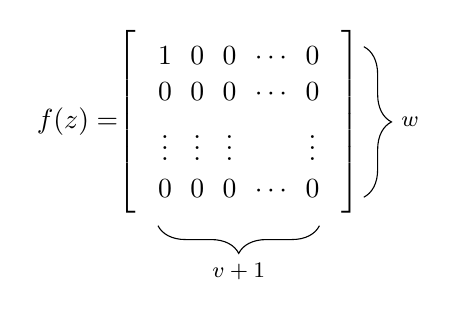
\begin{tikzpicture}
 \matrix (vec) [matrix of math nodes, left delimiter = {[}, right delimiter = {]}] {
1 & 0 & 0 & \cdots & 0\\
0 & 0 & 0 & \cdots & 0\\
\vdots & \vdots & \vdots & & \vdots\\
0 & 0 & 0 & \cdots & 0\\
};
	
\node (a) at (vec-1-5.north) [right=15pt] {};
\node (d) at (vec-4-5.south) [right=15pt] {};
\draw [decorate, decoration={brace, amplitude=10pt}] (a)--(d) node[midway, right=10pt] {\footnotesize $w$};
	
\node (e) at (vec-4-1.center) [left=0pt] {};
\draw [] (e) node[midway, left=40pt] {$f(z) = $};
	
\node (f) at (vec-4-1.west) [below=10pt] {};
\node (i) at (vec-4-5.east) [below=10pt] {};
\draw [decorate, decoration={brace, amplitude=10pt}] (i)--(f) node[midway, below=10pt] {\footnotesize $v + 1$};
\end{tikzpicture}
\end{center}
	
那么对于任意 $\widehat{X} \in \mathbb{X}$，对应的 CDE 解在 $\mathcal{Z}$ 中是
\begin{equation*}
	z^{f, \zeta, X}_t = z^{f, \zeta, X}_{\tau} + \int_{\tau}^t f(z^{f, \zeta, X}_s) \mathrm{d}X_s,
\end{equation*}
因此其解的第一个分量是
\begin{equation*}
	z^{f, \zeta, X, 1}_t = X^1_t-X^1_\tau + \zeta^1(X_\tau),
\end{equation*}
而其他分量是常数
\begin{equation*}
	z^{f, \zeta, X, i}_t = \zeta^i(X_\tau)
\end{equation*}
对于 $i \in \{2, \ldots, w\}$，其中上标表示分量。
	
现在假设存在矛盾，即存在 $y^{h, \zeta, \cdot} \in \mathcal{Y}$ 对于某些 $\Xi \in \xi$ 和 $h \in H$ 使得 $y^{h, \Xi, X} = \pi \circ z^{f, \zeta, X}$ 对所有 $\widehat{X} \in \mathbb{X}$ 成立。那么 $y^{h, \Xi, X}$ 必须满足
\begin{equation*}
	y^{h, \Xi, X}_t = y^{h, \Xi, X}_\tau + \int_\tau^t h(y^{h, \Xi, X}_s, X_s) \mathrm{d}s,
\end{equation*}
因此
\begin{equation*}
	(X^1_t-X^1_{\tau} + \zeta^1(X_\tau), 0, \ldots, 0) = \pi(\Xi(X_\tau)) + \int_{\tau}^t h((X^1_s-X^1_{\tau} + \zeta^1(X_\tau), \zeta^2(X_\tau), \ldots, \zeta^w(X_\tau)), X_s) \mathrm{d}s.
\end{equation*}
考虑那些可微的 $X$。对 $t$ 求导得到
\begin{equation}\label{eq:impossible}
	\frac{\mathrm{d}X^1}{\mathrm{d}t}(t) = h^1((X^1_s-X^1_{\tau} + \zeta^1(X_\tau), \zeta^2(X_\tau), \ldots, \zeta^w(X_\tau)), X_t).
\end{equation}
	
也就是说，$h^1$ 满足方程 \eqref{eq:impossible} 对所有可微的 $X$EQU_8005748E__

	也就是说，$h^1$ 对于所有可微的 $X$ 满足方程 \eqref{eq:impossible}。这显然是不可能的：右边只是 $t$、$X_t$ 和 $X_{\tau}$ 的函数，不足以确定 $\ttfrac{\mathrm{d}X^1}{\mathrm{d}t}(t)$。

	\boldheading{$\mathcal{Y} \subseteq \mathcal{Z}$：}
	设对于某些 $\Xi \in \xi$ 和 $h \in H$ 有 $y^{h, \Xi, X} \in \mathcal{Y}$。令 $\sigma \colon \reals^w \to \reals^{v + 1}$ 是到最后 $v + 1$ 坐标的正交投影。设 $\zeta \in \xi$ 满足 $\pi \circ \zeta = \pi \circ \Xi$ 且 $\sigma(\zeta(X_\tau)) = X_\tau$。然后定义 $f \in F$ 如下
\begin{center}
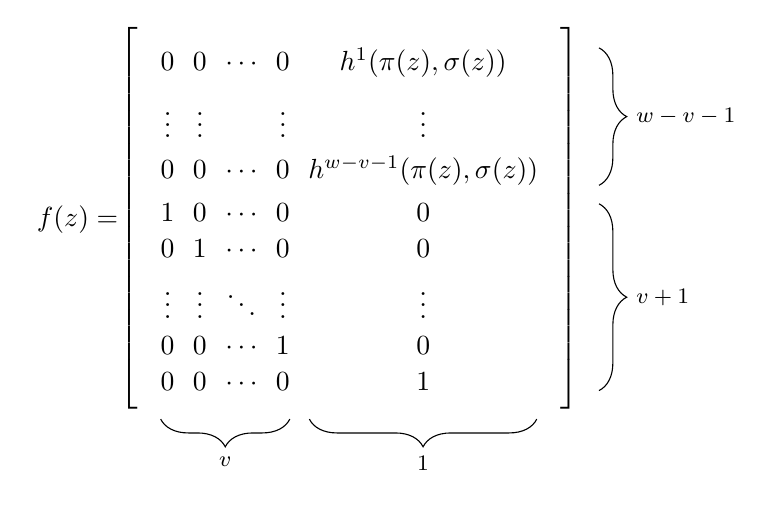
\begin{tikzpicture}
	 \matrix (vec) [matrix of math nodes, left delimiter = {[}, right delimiter = {]}] {
	0 & 0 & \cdots & 0 & h^1(\pi(z), \sigma(z))\\
	\vdots & \vdots & & \vdots & \vdots\\
	0 & 0 & \cdots & 0 & h^{w-v-1}(\pi(z), \sigma(z))\\
	1 & 0 & \cdots & 0 & 0\\
	0 & 1 & \cdots & 0 & 0\\
	\vdots & \vdots & \ddots & \vdots & \vdots\\
	0 & 0 & \cdots & 1 & 0\\
	0 & 0 & \cdots & 0 & 1\\
	};
	
	\node (a) at (vec-1-5.north) [right=60pt] {};
	\node (b) at (vec-3-5.south) [right=60pt] {};
	\node (c) at (vec-4-5.north) [right=60pt] {};
	\node (d) at (vec-8-5.south) [right=60pt] {};
	\draw [decorate, decoration={brace, amplitude=10pt}] (a)--(b) node[midway, right=10pt] {\footnotesize $w-v-1$};
	\draw [decorate, decoration={brace, amplitude=10pt}] (c)--(d) node[midway, right=10pt] {\footnotesize $v + 1$};
	
	\node (e) at (vec-4-1.center) [left=0pt] {};
	\draw [] (e) node[midway, left=80pt] {$f(z) = $};
	
	\node (f) at (vec-8-1.west) [below=10pt] {};
	\node (g) at (vec-8-4.east) [below=10pt] {};
	\node (h) at (vec-8-4.east) [below=10pt] {};
	\node (i) at (vec-8-5.east) [below=10pt] {};
	\draw [decorate, decoration={brace, amplitude=10pt}] (g)--(f) node[midway, below=10pt] {\footnotesize $v$};
	\draw [decorate, decoration={brace, amplitude=10pt}] (i) + (35pt,0)--(h) node[midway, below=10pt] {\footnotesize $1$};
\end{tikzpicture}
\end{center}

	那么对于 $t \in (\tau, T]$，
\begin{align*}
	z^{f, \zeta, X}_t &= \zeta(X_\tau) + \int_\tau^t f(z^{f, \zeta, X}_s) \mathrm{d}X_s\\
	&=\zeta(X_\tau) + \int_\tau^t
\begin{bmatrix}
	0 & 0 & \cdots & 0 & h^1(\pi(z^{f, \zeta, X}_s), \sigma(z^{f, \zeta, X}_s))\\
	\vdots & \vdots & & \vdots & \vdots\\
	0 & 0 & \cdots & 0 & h^{w-v-1}(\pi(z^{f, \zeta, X}_s), \sigma(z^{f, \zeta, X}_s))\\
	1 & 0 & \cdots & 0 & 0\\
	0 & 1 & \cdots & 0 & 0\\
	\vdots & \vdots & \ddots & \vdots & \vdots\\
	0 & 0 & \cdots & 1 & 0\\
	0 & 0 & \cdots & 0 & 1\\
\end{bmatrix}
\begin{bmatrix}
	\mathrm{d}\widehat{X}^1_s\\
	\vdots\\
	\mathrm{d}\widehat{X}^v_s\\
	\mathrm{d}s
\end{bmatrix}\\
	&= \zeta(X_\tau) + \int_\tau^t
\begin{bmatrix}
	h^1(\pi(z^{f, \zeta, X}_s), \sigma(z^{f, \zeta, X}_s)) \mathrm{d}s\\
	\vdots\\
	h^{w-v-1}(\pi(z^{f, \zeta, X}_s), \sigma(z^{f, \zeta, X}_s)) \mathrm{d}s\\
	\mathrm{d}\widehat{X}^1_s\\
	\vdots\\
	\mathrm{d}\widehat{X}^v_s\\
	\mathrm{d}s\\
\end{bmatrix}\\
	&= \zeta(X_\tau) + \int_\tau^t
\begin{bmatrix}
	h(\pi(z^{f, \zeta, X}_s), \sigma(z^{f, \zeta, X}_s)) \mathrm{d}s\\
	\mathrm{d}X_s
\end{bmatrix}.
\end{align*}
	
	因此特别地
\begin{equation*}
	\sigma(z^{f, \zeta, X}_t) = \sigma(\zeta(X_\tau)) + \int_\tau^t \mathrm{d}X_s = \sigma(\zeta(X_\tau))-X_\tau + X_t = X_t.
\end{equation*}
	因此
\begin{equation*}
	\pi(z^{f, \zeta, X}_t) = \pi(\zeta(X_\tau)) + \int_\tau^t h(\pi(z^{f, \zeta, X}_s), \sigma(z^{f, \zeta, X}_s)) \mathrm{d}s  = \pi(\Xi(X_\tau)) + \int_\tau^t h(\pi(z^{f, \zeta, X}_s), X_s) \mathrm{d}s.
\end{equation*}
	
	因此我们看到 $\pi(z^{f, \zeta, X})$ 满足与 $y^{h, \Xi, X}$ 相同的微分方程。所以根据解的唯一性 \cite[Theorem 1.3]{levy-lyons}，$y^{h, \Xi, X} = \pi(z^{f, \zeta, X}) \in \mathcal{Z}$。
\end{proof}
	
	\section{实验细节}\label{appendix:experimental-details}
	
	\subsection{一般说明}
	\boldheading{代码}
	可以在 \url{https://github.com/patrick-kidger/NeuralCDE} 找到重现每个实验的代码。
	
	\boldheading{归一化}
	每个数据集都进行了归一化处理，使得每个通道的均值为零，方差为一。
	
	\boldheading{损失函数}
	每个二分类问题使用了对模型输出进行 sigmoid 处理后的二元交叉熵损失。每个多分类问题使用了对模型输出进行 softmax 处理后的交叉熵损失。分类问题使用了交叉熵损失应用于模型输出的softmax。

	\boldheading{架构}
	对于Neural CDE和ODE-RNN，被积函数$f_\theta$采用了一个前馈神经网络。总是使用一个最终的线性层将终端隐藏状态映射到输出。
	
	\boldheading{激活函数}
	对于Neural CDE模型，我们使用了ReLU激活函数。根据\cite{latent-odes}的建议，我们在ODE-RNN模型中使用了tanh激活函数，他们指出对于ODE-RNN模型，tanh激活似乎使模型更容易被ODE求解器解析。有趣的是，当我们尝试在Neural CDE模型中使用tanh激活和\texttt{method=`dopri5'}时，并没有观察到这种行为，因此我们选择了ReLU。
	
	\boldheading{优化器}
	每个问题都使用了由PyTorch 1.3.1 \cite{pytorch}实现的Adam \cite{kingma2015}优化器。学习率和批量大小在不同实验之间有所不同，请参见下文。如果指标在一定数量的epoch内未能改善，则降低学习率；如果指标在更大数量的epoch内未能改善，则终止训练。这些细节因实验而异，请参阅各个部分。一旦训练完成，参数就会回滚到在整个训练过程中产生最佳验证准确性的参数。最终线性层（从模型的隐藏状态映射到输出）的学习率通常比模型其他部分使用的要大得多；这是一个标准技巧，我们发现它提高了所有模型的性能。
	
	\boldheading{超参数选择}
	简而言之，超参数的选择是为了优化ODE-RNN基线，并为其他模型使用等效的超参数。
	
	更详细地说：
	
	我们首先选择了学习率。通过从0.001开始并逐渐减小直到小型ODE-RNN模型（批量大小为32）达到良好性能为止来选择学习率。
	
 在此之后，我们增加了批量大小，直到选定的模型以我们认为合理速度进行训练。按照惯例，随着批量大小的增加，我们也按比例增加了学习率。
	
 随后，我们通过网格搜索选择了模型超参数（隐藏通道的数量、向量场网络的宽度和深度），以优化ODE-RNN基线。对每个超参数选择执行了一次运行。然后，在调整以产生大致相同数量的参数后，将等效的超参数用于GRU-$\Delta$t、GRU-D、GRU-ODE基线以及我们的Neural CDE模型。
	
 搜索的网格及结果超参数在下面的各个部分中给出。
	
	\boldheading{权重正则化}
	$L^2$权重正则化应用于ODE-RNN、GRU-$\Delta$t和GRU-D模型的每个参数，以及Neural CDE和GRU-ODE模型的向量场的所有参数。
	
	\boldheading{ODE求解器}
	ODE-RNN、GRU-ODE和Neural CDE模型中的ODE组件都是使用四阶Runge-Kutta与3/8规则求解器计算的，这是通过向\texttt{torchdiffeq} \cite{torchdiffeq}包的\texttt{odeint\_adjoint}函数传递\texttt{method=`rk4'}实现的。传递给 \texttt{torchdiffeq} \cite{torchdiffeq} 包的 \texttt{odeint\_adjoint} 函数。步长被设置为任意两个相邻观测值之间的时间差的最小值。

\boldheading{伴随反向传播}
GRU-ODE、神经CDE以及ODE-RNN的ODE组件都是通过伴随反向传播方法 \cite{neural-odes} 进行训练的，该方法由 \texttt{torchdiffeq} 包中的 \texttt{odeint\_adjoint} 函数实现。

\boldheading{计算基础设施}
所有实验都在两台计算机中的一台上运行；这两台计算机都使用了Ubuntu 18.04.4 LTS，运行PyTorch 1.3.1，并使用了版本0.0.1的 \texttt{torchdiffeq} \cite{torchdiffeq} 包。其中一台计算机配备了Xeon E5-2960 v4处理器、两张GeForce RTX 2080 Ti显卡和两张Quadro GP100显卡，而另一台则配备了Xeon Silver 4104处理器和三张GeForce RTX 2080 Ti显卡。o Quadro GP100，而另一台则配备了Xeon Silver 4104和三块GeForce RTX 2080 Ti。

	\subsection{CharacterTrajectories}\label{appendix:uea}
	所使用的学習率是0.001，批次大小为32。如果验证损失在10个周期内停滞不前，则将学习率除以10并继续训练。如果训练损失或训练准确率在50个周期内停滞不前，则终止训练。允许的最大周期数为1000。
	
	我们将原始数据集的训练/测试分割（这些分割比例非常不寻常，为50\%/50\%）合并，然后采取了70\%/15\%/15\%的训练/验证/测试分割。
	
	神经CDE模型的初始条件$\zeta_\theta$被设定为从第一次观测到隐藏状态向量的一个学习线性映射。（回想一下，这是模型的重要组成部分，以避免平移不变性。）
	
	通过执行大部分网格搜索来优化超参数（仅针对之前描述的ODE-RNN基线），搜索范围包括16或32个隐藏通道、32、48、64、128个隐藏层大小以及1、2、3个隐藏层。（后两个超参数对应于ODE-RNN和神经CDE模型的向量场。）由于某些组合表现不佳，因此未测试一些选项组合。（例如，所有隐藏层大小为128的组合都表现出相对较差的性能。）该搜索仅在30\%缺失数据的情况下进行，并且对于50\%和70\%缺失数据的情况使用相同的超参数。
	
	选择的超参数为：神经CDE和ODE-RNN模型使用32个隐藏通道，GRU-$\Delta$t、GRU-D和GRU-ODE模型使用47个隐藏通道。神经CDE和ODE-RNN模型均使用前馈网络作为其向量场，每个宽度为32的隐藏层有3层。每种模型的结果参数计数分别为：神经CDE为8212，ODE-RNN为8436，GRU-D为8386，GRU-$\Delta$t为8292，GRU-ODE为8372。
	
	\subsection{PhysioNet sepsis prediction}\label{appendix:sepsis}
	所使用的批次大小为1024，学习率为0.0032，如前所述确定。如果训练损失在10个周期内停滞不前，则将学习率除以10并继续训练。如果训练损失或验证准确率在100个周期内停滞不前，则终止训练。允许的最大周期数为200。最终线性层的学习率（每个模型的一部分，从最终隐藏状态映射到输出）使用的是大100倍的学习率，即0.32。
	
	原始数据集没有现成的分割，因此我们自己采用了70\%/15\%/15\%的训练/验证/测试分割。
	
	由于这个问题包含了静态（非时变）特征，我们通过让每个模型的初始条件依赖于这些信息来整合这些信息。这被设定为一个具有ReLU激活函数且宽度为256的单隐藏层前馈网络，我们并未对其进行超参数搜索。
	
	由于此数据集部分观察，对于需要在每个时间步骤传递某些内容的ODE-RNN、GRU-$\Delta$t、GRU-D模型，即使值缺失，我们也用自然三次样条填充缺失值，以便与神经CDE和ODE-RNN模型进行比较。（我们不将其描述为插补，因为在观察强度情况下，观察掩码也会传递给这些模型。）特别是这与GRU-D的通常实现略有不同，后者通常使用最后一次观察值和平均值的加权平均。l 实现了GRU-D，通常使用最后一次观测值和均值的加权平均。样条函数实现了几乎相同的功能，并有助于在各种模型之间保持一致性。
	
	通过在64、128、256隐藏通道，64、128、256隐藏层大小以及1、2、3、4隐藏层上进行大部分网格搜索来优化超参数（仅针对之前描述的ODE-RNN基线）。（后两个超参数对应于ODE-RNN和Neural CDE模型的向量场。）
	
	为ODE-RNN模型选择的超参数是128个隐藏通道，以及由具有128个隐藏层大小和4个隐藏层的前馈神经网络给出的向量场。为了使每个模型之间的参数数量相同，对于Neural CDE模型，这被减少到49个隐藏通道和49个隐藏层大小，而对于GRU-$\Delta$t、GRU-D和GRU-ODE模型，则增加到187个隐藏通道。当使用观测强度时，结果参数计数分别为：Neural CDE为193541，ODE-RNN为194049，GRU-D为195407，GRU-$\Delta$t为195033，GRU-ODE为194541。当不使用观测强度时，结果参数计数分别为：Neural CDE为109729，ODE-RNN为180097，GRU-D为175260，GRU-$\Delta$t为174886，GRU-ODE为174921。请注意Neural CDE的显著减少的参数计数；这是因为移除观测强度减少了通道数量，从而如第\ref{section:limitations}节所述显著影响了参数计数。
	
	\subsection{语音命令}\label{appendix:speechcommands}
	使用的批量大小为1024，学习率为0.0016，这是按照先前描述的方式确定的。如果训练损失停滞10个周期，则将学习率除以10并恢复训练。如果训练损失或验证准确率停滞100个周期，则终止训练。允许的最大周期数为200。最终线性层的学习率（每个模型的一个组成部分，从最终隐藏状态映射到输出）使用的是大100倍的学习率，即0.16。
	
	数据集中的每个时间序列都是单变量且长度为16000。我们计算了输入的20个Mel频率倒谱系数，如\texttt{torchaudio.transforms.MFCC}实现的那样，并对系数应用了对数缩放。短时傅里叶变换组件的窗口是一个长度为200的Hann窗口，跳跃长度为100，有200个频率箱。这通过了128个mel滤波器组，并提取了20个mel系数。这产生了一个长度为161、具有20个通道的时间序列。我们采用了70\%/15\%/15\%的训练/验证/测试划分。
	
	通过在32、64、128隐藏通道，32、64、128隐藏层大小以及1、2、3、4隐藏层上进行大部分网格搜索来优化超参数（仅针对之前描述的ODE-RNN基线）。（后两个超参数对应于ODE-RNN和Neural CDE模型的向量场。）
	
	为ODE-RNN模型选择的超参数是128个隐藏通道，以及由具有64个隐藏层大小和4个隐藏层的前馈神经网络给出的向量场。为了使每个模型之间的参数数量相同，对于Neural CDE模型，这被减少到90个隐藏通道和40个隐藏层大小，而对于GRU-$\Delta$t、GRU-D和GRU-ODE模型，则增加到160个隐藏通道。结果参数计数分别为：Neural CDE模型为88940，ODE-RNN模型为87946，GRU-D模型为89290，GRU-dt模型为88970，GRU-ODE模型为89180。
\end{document}